\documentclass[red]{beamer}
%\documentclass[handout]{beamer}

\usepackage{fixltx2e}
\usepackage{movie15}
\usepackage{hyperref}

%\usepackage[usenames,dvipsnames]{color}
%\usepackage[english]{babel}
\usepackage{tabularx}
\usepackage{soul}
\usepackage{xparse}
\usepackage{listings}


%%%%%%%%%%%%%%%
% Show a list of items "todo" or "done" 
% USAGE: 
% \begin{todolist} 
% 	\todo Something not finished
% 	\done Something finished
% \end{todolist} 
\newenvironment{todolist}{%
  \begin{list}{}{}% whatever you want the list to be
  \let\olditem\item
  \renewcommand\item{\olditem \textcolor{red}{(TODO)}: }
  \newcommand\todo{\olditem \textcolor{red}{(TODO)}: }
   \newcommand\done{\olditem \textcolor{ForestGreen}{(DONE)}: }
}{%
  \end{list}
} 
%%%%%%%%%%%%%%%



%%%%%%%%%%%%%%%
% Show a Author's Note
% USAGE: 
% \authnote[Optional footnote message to further clarify note]{The note to your readers}
\DeclareDocumentCommand \authnote { o m }
{%
\IfNoValueTF {#1}
{\textcolor{blue}{Author's Note: \uline{#2}}} 
{\textcolor{blue}{Author's Note: \uline{#2}}\footnote{Comment: #1}}%
{\textcolor{red}{Gordon's Note: \uline{#2}}\footnote{Comment: #1}}%
}
%%%%%%%%%%%%%%%



%%%%%%%%%%%%%%%
% Strike out text that doesn't belong in the paper
% USAGE: 
% \strike[Optional footnote to state why it doesnt belong]{Text to strike out}
\DeclareDocumentCommand \strike { o m }
{%
\IfNoValueTF {#1}
{\textcolor{red}{\sout{#2}}} 
{\textcolor{red}{\sout{#2}}\footnote{Comment: #1}}%
}
%%%%%%%%%%%%%%%

\definecolor{light-gray}{gray}{0.95}

\newcommand{\cbox}[3]{
\ \\
\fcolorbox{#1}{#2}{
\parbox{\textwidth}{
#3
}
}
}

% Setup an environment similar to verbatim but which will highlight any bash commands we have
\lstnewenvironment{unixcmds}[0]
{
%\lstset{language=bash,frame=shadowbox,rulesepcolor=\color{blue}}
\lstset{ %
language=sh,		% Language
basicstyle=\ttfamily,
backgroundcolor=\color{light-gray}, 
rulecolor=\color{blue},
%frame=tb, 
columns=fullflexible,
%framexrightmargin=-.2\textwidth,
linewidth=0.8\textwidth,
breaklines=true,
%prebreak=/, 
  prebreak = \raisebox{0ex}[0ex][0ex]{\ensuremath{\hookleftarrow}},
%basicstyle=\footnotesize,       % the size of the fonts that are used for the code
%numbers=left,                   % where to put the line-numbers
%numberstyle=\footnotesize,      % the size of the fonts that are used for the line-numbers
%stepnumber=2,                   % the step between two line-numbers. If it's 1 each line 
                                % will be numbered
%numbersep=5pt,                  % how far the line-numbers are from the code
showspaces=false,               % show spaces adding particular underscores
showstringspaces=false,         % underline spaces within strings
showtabs=false,                 % show tabs within strings adding particular underscores
frame=single,	                % adds a frame around the code
tabsize=2,	                % sets default tabsize to 2 spaces
captionpos=b,                   % sets the caption-position to bottom
breakatwhitespace=false,        % sets if automatic breaks should only happen at whitespace
}
} { }

% Setup an environment similar to verbatim but which will highlight c++ syntax
\lstnewenvironment{cppcode}[1]
{
%\lstset{language=bash,frame=shadowbox,rulesepcolor=\color{blue}}
\lstset{ %
	backgroundcolor=\color{light-gray},
	rulecolor=\color[rgb]{0.133,0.545,0.133},
	tabsize=4,
	language=[GNU]C++,
%	basicstyle=\ttfamily,
        basicstyle=\scriptsize,
        upquote=true,
        aboveskip={1.5\baselineskip},
        %columns=fullflexible,
        %framexrightmargin=-.1\textwidth,
       %framexleftmargin=6mm,
        showstringspaces=false,
        extendedchars=true,
        breaklines=true,
        prebreak = \raisebox{0ex}[0ex][0ex]{\ensuremath{\hookleftarrow}},
        frame=single,
        showtabs=false,
        tabsize=4,
        showspaces=false,
        showstringspaces=false,
        numbers=left,                   % where to put the line-numbers
        numbers=none,                   % where to put the line-numbers
	numberstyle=\footnotesize,      % the size of the fonts that are used for the line-numbers
	stepnumber=4,                   % the step between two line-numbers. If it's 1 each line 
                                % will be numbered
	firstnumber=#1,
         numbersep=5pt,                  % how far the line-numbers are from the code
        identifierstyle=\ttfamily,
        keywordstyle=\color[rgb]{0,0,1},
        commentstyle=\color[rgb]{0.133,0.545,0.133},
        stringstyle=\color[rgb]{0.627,0.126,0.941},
}
} { }

% Setup an environment similar to verbatim but which will highlight any bash commands we have
\lstnewenvironment{mcode}[1]
{
\lstset{ %
	backgroundcolor=\color{light-gray}, 
	rulecolor=\color[rgb]{0.133,0.545,0.133},
	tabsize=4,
	language=Matlab,
%	basicstyle=\ttfamily,
        basicstyle=\scriptsize,
        upquote=true,
        aboveskip={1.5\baselineskip},
        columns=fullflexible,
        %framexrightmargin=-.1\textwidth,
       %framexleftmargin=6mm,
        showstringspaces=false,
        extendedchars=true,
        breaklines=true,
        prebreak = \raisebox{0ex}[0ex][0ex]{\ensuremath{\hookleftarrow}},
        frame=single,
        showtabs=false,
        showspaces=false,
        showstringspaces=false,
        numbers=left,                   % where to put the line-numbers
	numberstyle=\footnotesize,      % the size of the fonts that are used for the line-numbers
	stepnumber=4,                   % the step between two line-numbers. If it's 1 each line 
                                % will be numbered
	firstnumber=#1,
         numbersep=5pt,                  % how far the line-numbers are from the code
        identifierstyle=\ttfamily,
        keywordstyle=\color[rgb]{0,0,1},
        commentstyle=\color[rgb]{0.133,0.545,0.133},
        stringstyle=\color[rgb]{0.627,0.126,0.941},
}
} { }

\newcommand{\inputmcode}[1]{%
\lstset{ %
	backgroundcolor=\color{light-gray},  %
	rulecolor=\color[rgb]{0.133,0.545,0.133}, %
	tabsize=4, %
	language=Matlab, %
%	basicstyle=\ttfamily,
        basicstyle=\scriptsize, %
        %        upquote=true,
        aboveskip={1.5\baselineskip}, %
        columns=fullflexible, %
        %framexrightmargin=-.1\textwidth,
       %framexleftmargin=6mm,
        showstringspaces=false, %
        extendedchars=true, %
        breaklines=true, %
        prebreak = \raisebox{0ex}[0ex][0ex]{\ensuremath{\hookleftarrow}}, %
        frame=single, %
        showtabs=false, %
        showspaces=false, %
        showstringspaces=false,%
        numbers=left,                   % where to put the line-numbers
	numberstyle=\footnotesize,      % the size of the fonts that are used for the line-numbers
	stepnumber=4,                   % the step between two line-numbers. If it's 1 each line 
                                % will be numbered
         numbersep=5pt,                  % how far the line-numbers are from the code
        identifierstyle=\ttfamily, %
        keywordstyle=\color[rgb]{0,0,1}, %
        commentstyle=\color[rgb]{0.133,0.545,0.133}, %
        stringstyle=\color[rgb]{0.627,0.126,0.941} %
}
\lstinputlisting{#1}%
}

%\lstset{ %
%	backgroundcolor=\color{light-gray}, 
%	rulecolor=\color[rgb]{0.133,0.545,0.133},
%	tabsize=4,
%	language=Matlab,
%%	basicstyle=\ttfamily,
%        basicstyle=\scriptsize,
%        upquote=true,
%        aboveskip={1.5\baselineskip},
%        columns=fullflexible,
%        %framexrightmargin=-.1\textwidth,
%       %framexleftmargin=6mm,
%        showstringspaces=false,
%        extendedchars=true,
%        breaklines=true,
%        prebreak = \raisebox{0ex}[0ex][0ex]{\ensuremath{\hookleftarrow}},
%        frame=single,
%        showtabs=false,
%        showspaces=false,
%        showstringspaces=false,
%        numbers=left,                   % where to put the line-numbers
%	numberstyle=\footnotesize,      % the size of the fonts that are used for the line-numbers
%	stepnumber=4,                   % the step between two line-numbers. If it's 1 each line 
%                                % will be numbered
%	firstnumber=#1,
%         numbersep=5pt,                  % how far the line-numbers are from the code
%        identifierstyle=\ttfamily,
%        keywordstyle=\color[rgb]{0,0,1},
%        commentstyle=\color[rgb]{0.133,0.545,0.133},
%        stringstyle=\color[rgb]{0.627,0.126,0.941},
%}


\newcommand{\Laplacian}[1]{\nabla^2 #1}

% set of all nodes received and contained on GPU
\newcommand{\setAllNodes}[0]{\mathcal{G}}
% set of stencil centers on GPU
\newcommand{\setCenters}[0]{\mathcal{Q}}
% set of stencil centers with nodes in \setDepend
\newcommand{\setBoundary}[0]{\mathcal{B}}
% set of nodes received by other GPUs
\newcommand{\setDepend}[0]{\mathcal{R}}
% set of nodes sent to other GPUs
\newcommand{\setProvide}[0]{\mathcal{O}}


\newcommand{\toprule}[0]{\hline}
\newcommand{\midrule}[0]{\hline\hline}
\newcommand{\bottomrule}[0]{\hline}

\newcolumntype{C}{>{\centering\arraybackslash}b{1in}}
\newcolumntype{L}{>{\flushleft\arraybackslash}b{1.5in}}
\newcolumntype{R}{>{\flushright\arraybackslash}b{1.5in}}
\newcolumntype{D}{>{\flushright\arraybackslash}b{2.0in}}
\newcolumntype{E}{>{\flushright\arraybackslash}b{1.0in}}

\DeclareSymbolFont{AMSb}{U}{msb}{m}{n}
\DeclareMathSymbol{\N}{\mathbin}{AMSb}{"4E}
\DeclareMathSymbol{\Z}{\mathbin}{AMSb}{"5A}
\DeclareMathSymbol{\R}{\mathbin}{AMSb}{"52}
\DeclareMathSymbol{\Q}{\mathbin}{AMSb}{"51}
\DeclareMathSymbol{\PP}{\mathbin}{AMSb}{"50}
\DeclareMathSymbol{\I}{\mathbin}{AMSb}{"49}
\DeclareMathSymbol{\C}{\mathbin}{AMSb}{"43}

%%%%%% VECTOR NORM: %%%%%%%
\newcommand{\vectornorm}[1]{\left|\left|#1\right|\right|}
%\renewcommand{\vec}[1]{ \textbf{#1} }
%%%%%%%%%%%%%%%%%%%%%%

%%%%%%% THM, COR, DEF %%%%%%%
%\newtheorem{theorem}{Theorem}[section]
%\newtheorem{lemma}[theorem]{Lemma}
%\newtheorem{proposition}[theorem]{Proposition}
%\newtheorem{corollary}[theorem]{Corollary}
%\newenvironment{proof}[1][Proof]{\begin{trivlist}
%\item[\hskip \labelsep {\bfseries #1}]}{\end{trivlist}}
%\newenvironment{definition}[1][Definition]{\begin{trivlist}
%\item[\hskip \labelsep {\bfseries #1}]}{\end{trivlist}}
%\newenvironment{example}[1][Example]{\begin{trivlist}
%\item[\hskip \labelsep {\bfseries #1}]}{\end{trivlist}}
%\newenvironment{remark}[1][Remark]{\begin{trivlist}
%\item[\hskip \labelsep {\bfseries #1}]}{\end{trivlist}}
%\newcommand{\qed}{\nobreak \ifvmode \relax \else
%      \ifdim\lastskip<1.5em \hskip-\lastskip
%      \hskip1.5em plus0em minus0.5em \fi \nobreak
%      \vrule height0.75em width0.5em depth0.25em\fi}
%%%%%%%%%%%%%%%%%%%%%%

%
%\usepackage[algochapter]{algorithm2e}
%\usepackage[usenames]{color}
% colors to show the corrections
\newcommand{\red}[1]{\textbf{\textcolor{red}{#1}}}
\newcommand{\blue}[1]{\textbf{\textcolor{blue}{#1}}}
\newcommand{\cyan}[1]{\textbf{\textcolor{cyan}{#1}}}
\newcommand{\green}[1]{\textbf{\textcolor{green}{#1}}}
\newcommand{\magenta}[1]{\textbf{\textcolor{magenta}{#1}}}
\newcommand{\orange}[1]{\textbf{\textcolor{orange}{#1}}}
%%%%%%%%%% DK DK
% comments between authors
\newcommand{\toall}[1]{\textbf{\green{@@@ All: #1 @@@}}}
\newcommand{\toevan}[1]{\textbf{\red{*** Evan: #1 ***}}}
\newcommand{\toe}[1]{\textbf{\red{*** Evan: #1 ***}}}

% to Accept all edits, simply remove the color
\newcommand{\EDIT}[2]{\cyan{#1}}
\newcommand{\ED}[2]{\cyan{#1}}

\newcommand{\mmy}[1]{\textbf{\blue{*** To Myrna: #1 ***}}}
\newcommand{\toi}[1]{\textbf{\magenta{*** Ian: #1 ***}}}
\newcommand{\togordon}[1]{\textbf{\blue{*** Gordon: #1 ***}}}
\newcommand{\gee}[1]{{\bf{\blue{{\em #1}}}}}
\newcommand{\old}[1]{}
\newcommand{\del}[1]{***#1*** }



% \DeclareMathOperator{\Sample}{Sample}
%\let\vaccent=\v % rename builtin command \v{} to \vaccent{}
%\renewcommand{\vec}[1]{\ensuremath{\mathbf{#1}}} % for vectors
\newcommand{\gv}[1]{\ensuremath{\mbox{\boldmath$ #1 $}}} 
% for vectors of Greek letters
\newcommand{\uv}[1]{\ensuremath{\mathbf{\hat{#1}}}} % for unit vector
\newcommand{\abs}[1]{\left| #1 \right|} % for absolute value
\newcommand{\avg}[1]{\left< #1 \right>} % for average
\let\underdot=\d % rename builtin command \d{} to \underdot{}
\renewcommand{\d}[2]{\frac{d #1}{d #2}} % for derivatives
\newcommand{\dd}[2]{\frac{d^2 #1}{d #2^2}} % for double derivatives
\newcommand{\pd}[2]{\frac{\partial #1}{\partial #2}} 
% for partial derivatives
\newcommand{\pdd}[2]{\frac{\partial^2 #1}{\partial #2^2}} 
\newcommand{\pdda}[3]{\frac{\partial^2 #1}{\partial #2 \partial #3}} 
% for double partial derivatives
\newcommand{\pdc}[3]{\left( \frac{\partial #1}{\partial #2}
 \right)_{#3}} % for thermodynamic partial derivatives
\newcommand{\ket}[1]{\left| #1 \right>} % for Dirac bras
\newcommand{\bra}[1]{\left< #1 \right|} % for Dirac kets
\newcommand{\braket}[2]{\left< #1 \vphantom{#2} \right|
 \left. #2 \vphantom{#1} \right>} % for Dirac brackets
\newcommand{\matrixel}[3]{\left< #1 \vphantom{#2#3} \right|
 #2 \left| #3 \vphantom{#1#2} \right>} % for Dirac matrix elements
\newcommand{\grad}[1]{\gv{\nabla} #1} % for gradient
\let\divsymb=\div % rename builtin command \div to \divsymb
\renewcommand{\div}[1]{\gv{\nabla} \cdot #1} % for divergence
\newcommand{\curl}[1]{\gv{\nabla} \times #1} % for curl
\let\baraccent=\= % rename builtin command \= to \baraccent
\renewcommand{\=}[1]{\stackrel{#1}{=}} % for putting numbers above =
\newcommand{\diffop}[1]{\mathcal{L}#1}
\newcommand{\boundop}[1]{\mathcal{B}#1}
\newcommand{\rvec}[0]{{\bf r}}

\newcommand{\Interior}[0]{\Omega}
\newcommand{\Boundary}[0]{\partial \Omega}

\newcommand{\on}[1]{\hskip1.5em \textrm{ on } #1}

\newcommand{\gemm}{\texttt{GEMM}}
\newcommand{\trmm}{\texttt{TRMM}}
\newcommand{\gesvd}{\texttt{GESVD}}
\newcommand{\geqrf}{\texttt{GEQRF}}


\newcommand{\minitab}[2][l]{\begin{tabular}{#1}#2\end{tabular}}
\newcommand{\comm}[1]{\textcolor{red}{\textit{#1}}}

\newcommand{\nfrac}[2]{
\nicefrac{#1}{#2}
%\frac{#1}{#2}
}

%% Rename  this file          misc_mac.tex
%----------------------------------------------------------------------
%%%%%%%%%%%%%%%%%%%%%%%%%%%%%%%%%%%%%%%%%%%%%%%%%%%%%%%%%%%%%%%%%%%%%%%%%%%%%%%
%
%	Math Symbols   Math Symbols   Math Symbols   Math Symbols   
%
%%%%%%%%%%%%%%%%%%%%%%%%%%%%%%%%%%%%%%%%%%%%%%%%%%%%%%%%%%%%%%%%%%%%%%%%%%%%%%%
\def\pmb#1{\setbox0=\hbox{$#1$}%
	\kern-.025em\copy0\kern-\wd0
	\kern.05em\copy0\kern-\wd0
	\kern-.025em\raise.0433em\box0}
\def\pmbf#1{\pmb#1}
\def\bfg#1{\pmb#1}

% BETTER VALUES FOR AUTOMATIC FIGURE PLACEMENT THAN THOSE PROVIDED BY 
% LATEX DEFAULTS.

\renewcommand{\textfloatsep}{1ex}
\renewcommand{\floatpagefraction}{0.9}
\renewcommand{\intextsep}{1ex}
\renewcommand{\topfraction}{.9}
\renewcommand{\bottomfraction}{.9}
\renewcommand{\textfraction}{.1}

% #1  position of floating figure (h|t|b|p)
% #1  EPS postscript file
% #2  size
% #3  caption

%usage of newfig:
%  \newfig{file.ps}{3in}{Fig1: this is a figure}

\input{epsf}
\def\newfig#1#2#3{
  \begin{figure}[htbp]
  \vspace{1ex}
  \setlength{\epsfxsize}{#2}
  \centerline{\epsfbox{#1}}
  \vspace{-.1in}\caption{\small #3}\break\vspace{.2in}
  \label{#1}
  \end{figure}
}

%usage of newfigtwo: 2 figures, vertically stacked
% \newfig
%	{file1.ps}
%	{file2.ps}
%	{width}
%	{vertical space}
%	{Caption}

\def\newfigtwo#1#2#3#4#5{
  \begin{figure}[htbp]
  \vspace{1ex}
  \setlength{\epsfxsize}{#3}
  \centerline{\epsfbox{#1}}
  \vspace{#4}
  \setlength{\epsfxsize}{#3}
  \centerline{\epsfbox{#2}}
  \vspace{-.1in}\caption{\small #5}\break\vspace{.2in}
  \label{#1}
  \end{figure}
}

\def\newfigh#1#2#3#4{  % add height specification
  \begin{figure}[htbp]
  \vspace{1ex}
  \setlength{\epsfxsize}{#2}
  \setlength{\epsfysize}{#4}
  \centerline{\epsfbox{#1}}
  \vspace{-.1in}\caption{\small #3}\break\vspace{.2in}
  \label{#1}
  \end{figure}
}

\def\herefig#1#2#3{
  \begin{figure}[h]
  \setlength{\epsfxsize}{#2}
  \centerline{\epsfbox{#1}}
  \caption{\small #3}
  \label{#1}
  \end{figure}
}

\def\etal{{{\em et~al.\,\,}}}
\def\note#1{\\ =====#1===== \\}
\def\FBOX#1{\ \\ \fbox{\begin{minipage}{5in}#1\end{minipage}}\\ }
\newcount\sectionno     \sectionno=0
\newcount\eqnum         \eqnum=0
\def\addeqno{\global\advance \eqnum by  1 }
\def\subeqno{\global\advance \eqnum by -1 }
%\def\eqn{\addeqno \eqno \hbox{(\number\sectionno.\number\eqnum)} }

\def\tildetilde#1{\tilde{\tilde{#1}}}
\def\barbar#1{\overbar{\overbar{#1}}}

\def\vsp#1{\vspace{#1 ex}}
\def\fpar{\hspace{\parindent}}
%
%  \pf : 2 arguments: numerator and denominator of partial derivative
%
\def\pf#1#2{{\frac{\partial{#1}}{\partial{#2}}}}
\def\pfs#1#2{{\partial_{#2}{#1}}}
\def\pftwo#1#2{{\frac{\partial^2{#1}}{\partial{#2}^2}}}
\def\pfxx#1#2{{\frac{\partial^2{#1}}{\partial{#2}^2}}}
%\def\pfxy#1#2{{\frac{\partial^2{#1}}{\partial{#2}\partial{#3}}}}
\def\pfn#1#2#3{{\frac{\partial^{#1}{#2}}{\partial{#3}^{#1}}}}
\def\df#1#2{{\frac{d{#1}}{d{#2}}}}
\def\dfn#1#2#3{{\frac{d^{#1}{#2}}{d{#3}^{#1}}}}
\def\Dt#1#2{\frac{D#1}{D#2}}
\def\dt#1#2{\frac{d#1}{d#2}}
\def\bld#1{{\bf #1}}
\def\pfp#1#2#3{\pf{}{#3}{\left(\frac{#1}{#2}\right)}}

\def\norm#1{\|#1\|}

%
% Graphic characters  (\dot already defined by TeX/LateX)
%
\def\dash{\rule[1.5pt]{2mm}{.3mm}\HS{.9mm}}
\def\dott{\rule[1.5pt]{.7mm}{.3mm}\HS{.7mm}}
\def\dashline{\dash\dash\dash}
\def\dotline{\dott\dott\dott\dott\dott\dott}
\def\dashdotline{\dash$\cdot$\HS{.9mm}\dash}
\def\solidline{\rule[2pt]{7mm}{.3mm}}
% 
% overcircle
%
\def\ovcircle#1{\buildrel{\circ}\over{#1}}
%\def\below#1#2{\buildrel{#2}\under{#1}}
%\def\above#1#2{\buildrel{#2}\over{#1}}
%
%  big parenthesis and brackets
%
\def\bigpar#1#2{{\left(\frac{#1}{#2}\right)}}
\def\bigbra#1#2{{\left\[\frac{#1}{#2}\right\]}}

\def\Lp{\left(}
\def\Rp{\right)}
\def\Lb{\left[}
\def\Rb{\right]}
\def\Ln{\left\langle}
\def\Rn{\right\rangle}
\def\Ld{\left.}
\def\Rd{\right.}
\def\Lv{\left|}
\def\Rv{\right|}
\def\Lbr{\left|}
\def\Rbr{\right|}
\def\lng{\langle}
\def\rng{\rangle}
\def\Lc{\left\{}
\def\Rc{\right\}}
%%% %

% Cannot be handled by Lyx
%\def\[{{[}}
%\def\]{{]}}

%
\def\eol{\nonumber \\}
\def\eolnonb{\nonumber\\}
\def\eolnb{\\}
\def\nonb{\nonumber}
\def\be{\begin{equation}}
\def\ee{\end{equation}}
\def\BEQNA{\begin{eqnarray}}
\def\EEQNA{\end{eqnarray}}
\def\eqa{&=&}
\def\beqna{\begin{eqnarray}}
\def\eeqna{\end{eqnarray}}
\def\bverb{\begin{verbatim}}
\def\everb{\end{verbatim}}
\def\VERB#1{\bverb #1 \everb}
\def\btbl{\begin{tabular}}
\def\etbl{\end{tabular}}
\def\bmini{\begin{minipage}[t]{5.5in}}
\def\emini{\end{minipage}}
\def\parray#1#2{\left(\begin{array}{#1}#2\end{array}\right)}
\def\barray#1#2{\left[\begin{array}{#1}#2\end{array}\right]}
\def\carray#1#2{\left\{\begin{array}{#1}#2\end{array}\right.}
\def\darray#1#2{\left|\begin{array}{#1}#2\end{array}\right|}

\def\BEGTABLE#1{\begin{table}[hbt]\vspace{2ex}\begin{center}\bmini\centering\btbl{#1}}
\def\ENDTABLE#1#2{\etbl\caption[#1]{#2}\EMINI\end{center}\vspace{2ex}\end{table}}

\def\bfltbl#1{\begin{table}[hbt]\vspace{2ex}\begin{center}\bmini\centering\btbl{#1}}
\def\efltbl#1#2{\etbl\caption[#1]{#2}\emini\end{center}\vspace{2ex}\end{table}}
\def\mcol{\multicolumn}
%
%  label equations with (#)
%
\def\reff#1{(\ref{#1})}
%
%  macros borrowed from viewgraph package
%

\newenvironment{LETTRS}[3]{\begin{letter}{#1}
\input{origin}\opening{Dear #2:}\input{#3}\closing{Sincerely yours,}\end{letter}}{\clearpage}

\newenvironment{VIEW}[1]{{\BC\Huge\bf #1 \EC}\LARGE\VS{.05in}}{\clearpage}

\def\RM#1{\rm{#1\ }}
\def\BV{\begin{VIEW}}
\def\EV{\end{VIEW}}

\def\NI{\noindent}

\def\VS{\vspace*}
\def\HS{\hspace*}
\def\IT{\item}

\def\BARR{\begin{array}}
\def\EARR{\end{array}}

\def\BPARR{\left(\begin{array}}
\def\EPARR{\end{array}\right)}

\def\BDET{\left|\begin{array}}
\def\EDET{\end{array}\right|}

\def\BDF{\begin{definition}}
\def\EDF{\end{definition}}

\def\BSU{\begin{block}{Summary}}
\def\ESU{\end{block}}

\def\BEX{\begin{example}}
\def\EEX{\end{example}}

\def\BTH{\begin{theorem}}
\def\ETH{\end{theorem}}

\def\BCO{\begin{corollary}}
\def\ECO{\end{corollary}}

\def\BPROOF{\begin{proof}}
\def\EPROOF{\end{proof}}

\def\BLM{\begin{lemma}}
\def\ELM{\end{lemma}}

\def\BEQ{\begin{equation}}
\def\EEQ{\end{equation}}

\def\BEQNNB{$$}
\def\EEQNNB{$$}

\def\BE{\begin{enumerate}}
\def\EE{\end{enumerate}}

\def\BD{\begin{description}}
\def\ED{\end{description}}

\def\BI{\begin{itemize}}
\def\EI{\end{itemize}}

\def\BC{\begin{center}}
\def\EC{\end{center}}

\def\BFIG{\begin{figure}}
\def\EFIG{\end{figure}}

\def\BTABB{\begin{tabbing}}
\def\ETABB{\end{tabbing}}

\def\BMINI{\begin{minipage}}
\def\EMINI{\end{minipage}}

\def\BTABLE{\begin{table}}
\def\ETABLE{\end{table}}

\def\BTABUL{\begin{tabular}}
\def\ETABUL{\end{tabular}}

\def\MCOL{\multicolumn}
\def\UL{\underline}
\def\ULL#1{\UL{\UL{#1}}}

\def\BDOC{\begin{document}}
\def\EDOC{\end{document}}

\def\EM#1{{\em #1\/}}
\def\FN{\footnote}

% Courtesy of Ugo Piomelli

\def\latexfig #1 #2 #3 #4 #5 {\ \vfill
\hfill\hbox to 0.05in{\vbox to #3truein{
         \special{psfile="#1" angle=270 hscale=100 
                  hoffset=#4 voffset=#5 vscale=100} }\hfill}
\hfill\vspace{-0.1in}        }

% #1 is the .ps filename
% #2 is not used in the present version
% #3 is the size of the white space left above the caption (in inches)
% #4 is the horizontal offset from some unknown reference point.
%    It is in 1/72 of an inch and is positive to the right.
% #5 is the vertical offset from some unknown reference point.
%    It is in 1/72 of an inch and is positive upwards.



%\usetheme{MyTheme} 
%\usetheme{Berkeley}
\usetheme{Copenhagen}

% title
\title[Flocking Implementation for the Blender Game Engine]{Flocking Implementation for the Blender Game Engine}
\author{Myrna I. Merced Serrano}
\institute{\textbf{Adviser:} Dr. Gordon Erlebacher}
\date{June 24\textsuperscript{th}, 2011}

\setcounter{tocdepth}{1}

\begin{document}

%--------------------------------------------
% title 
%--------------------------------------------
\begin{frame}
	\titlepage
\end{frame}

%--------------------------------------------
% table of contents
%--------------------------------------------
\begin{frame}
	\tableofcontents
\end{frame}

%--------------------------------------------
% motivation - intro
%--------------------------------------------
\section{Motivation}

%--------------------------------------------
% educational games
%--------------------------------------------
\subsection{Educational Games}
\begin{frame}{Motivation}
	\begin{itemize}
		\pause \item Develop tools for educational games.
		\pause \item Address the poor performance in the basic classes of students.
		\pause \item Incorporate general tools such as flocking into public domain game engines.
	\end{itemize}	
\end{frame}

%--------------------------------------------
% related work
%--------------------------------------------
\subsection{Background and Related Work}

% flocking
\begin{frame}{Flocking}
	\begin{itemize}
		\pause \item \textit{Flocking} is a nature-inspired behavior, mostly seen in animals.
		\pause \item Collective motion of large group of entities. %, that exhibits interesting behavior as a whole.
	\end{itemize}
\end{frame}

\begin{frame}{Flocking}
	\begin{figure}[htbp]
	\begin{center}
	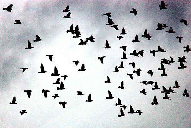
\includegraphics[scale=2.25]{figures/flock.pdf} 
	\end{center}
	\caption{Flocking behavior: Flock of birds}
	\label{default}
	\end{figure}

\end{frame}

\begin{frame}{Flocking}
	\begin{figure}[htbp]
	\begin{center}
	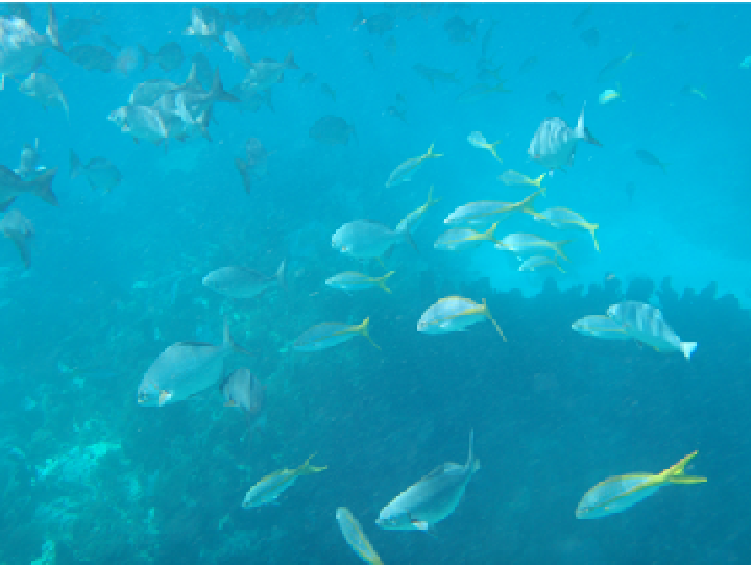
\includegraphics[scale=.55]{figures/school.pdf} 
	\end{center}
	\caption{Flocking behavior: Schooling}
	\label{default}
	\end{figure}

\end{frame}

\begin{frame}{Flocking}
	\begin{figure}[htbp]
	\begin{center}
	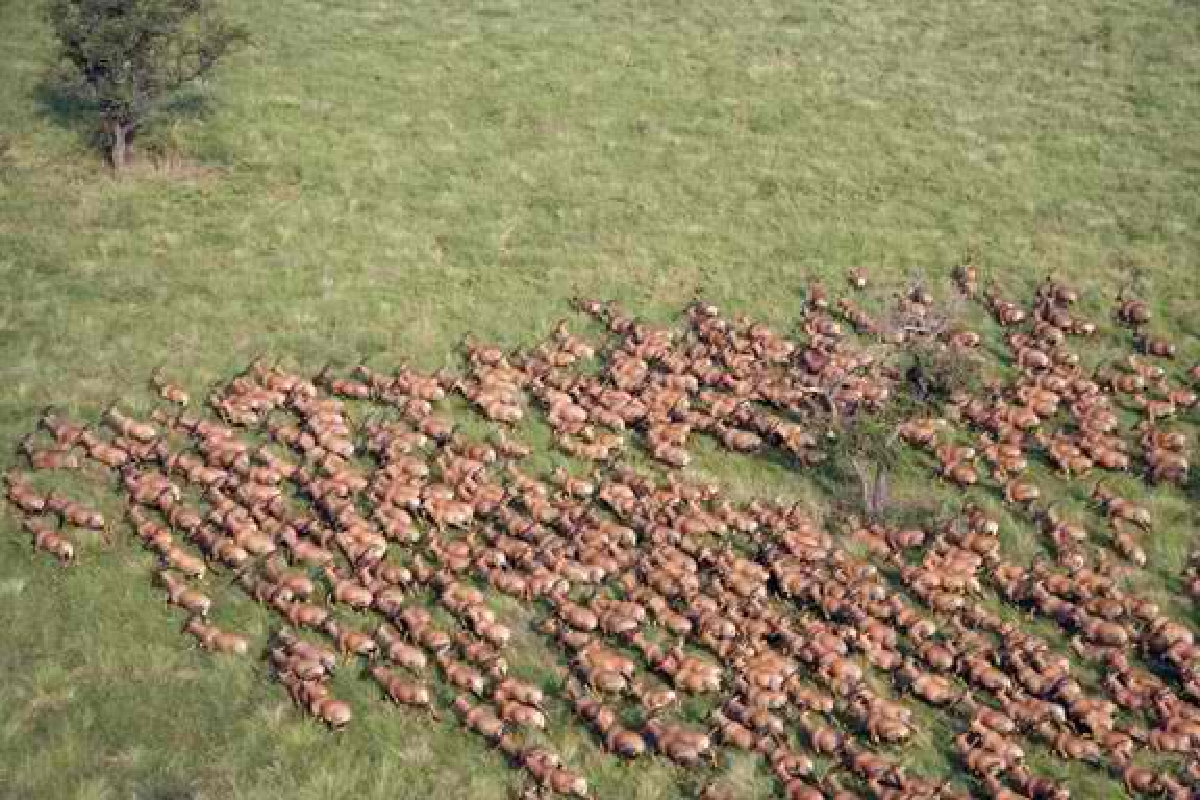
\includegraphics[scale=0.4]{figures/herd.pdf} 
	\end{center}
	\caption{Flocking behavior: Herd of quadrupeds}
	\label{default}
	\end{figure}

\end{frame}

\begin{frame}{Flocking}
	\begin{figure}[htbp]
	\begin{center}
	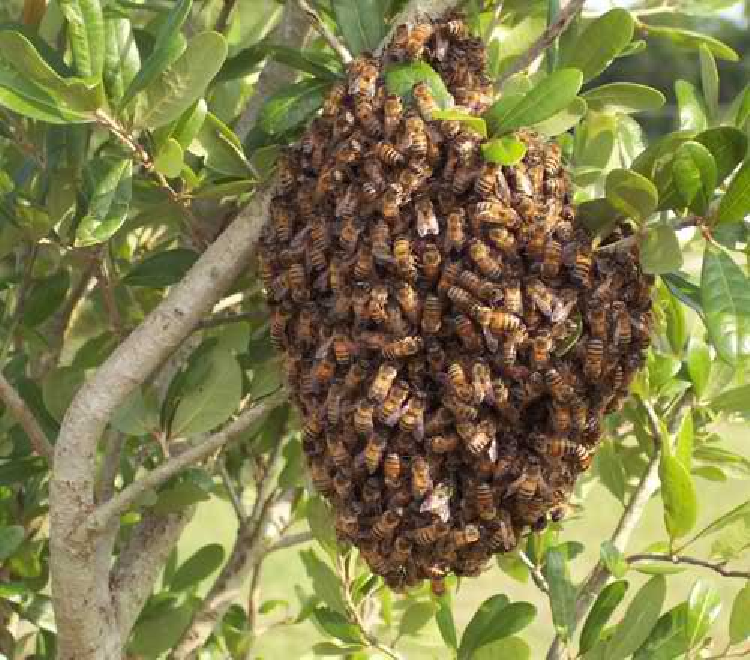
\includegraphics[scale=0.5]{figures/swarm.pdf}
	\end{center}
	\caption{Flocking behavior: Swarms of insects}
	\label{default}
	\end{figure}

\end{frame}


\begin{frame}{Craig Reynolds}
	\begin{itemize}
		\pause \item Craig Reynolds is the pioneer of flocking.
		\pause \item Inspired by the flocking behavior of birds he developed a behavioral model that simulates the self-organization of \textit{boids}.
		\pause \item \textit{Boids} are the entities of a flock.
		\pause \item Most recognized paper: \textit{Flocks, herds, and school: A Distributed Behavioral Model} revolutionized the field of flocking.
	\end{itemize}
\end{frame}

% craig
\begin{frame}{Original Boids Model by Craig Reynolds}
	\pause The set of rules, also called \textit{Boids Model}, consist of:
	
	\begin{columns}[b]
		\pause
		\begin{column}{4cm}
			\begin{figure}[htbp]
			\begin{center}
			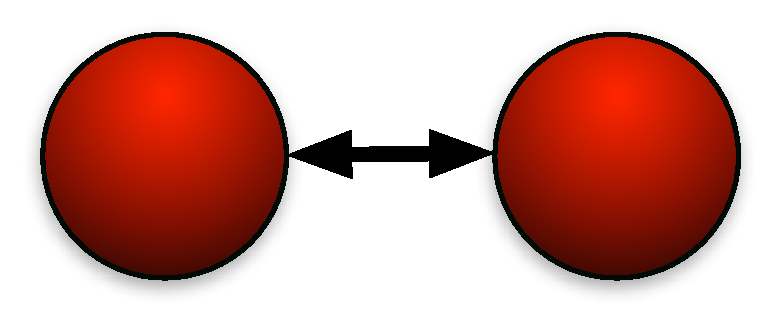
\includegraphics[scale=0.1]{../figures/sep_Craig.pdf}
			\caption{Collision Avoidance}
			\end{center}
			\end{figure}
		\end{column}
		\pause
		\begin{column}{4cm}
			\begin{figure}[htbp]
			\begin{center}
			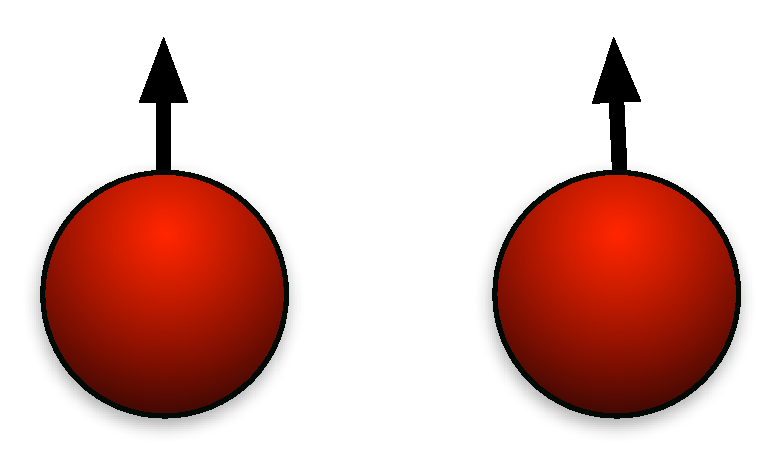
\includegraphics[scale=0.1]{../figures/align_Craig.pdf}
			\caption{Velocity Matching}
			\end{center}
			\end{figure}
		\end{column}
		\pause
		\begin{column}{4cm}
			\begin{figure}[htbp]
			\begin{center}
			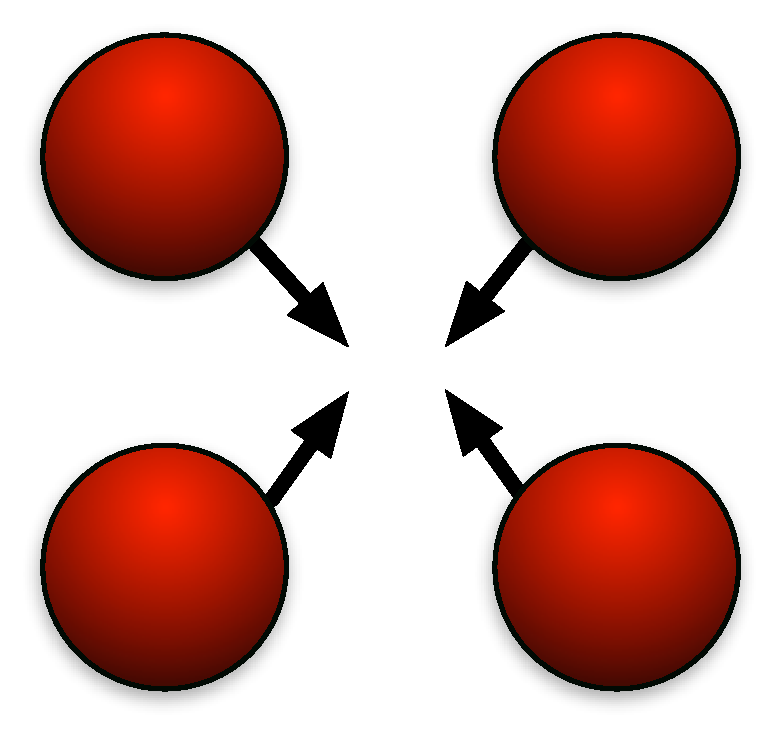
\includegraphics[scale=0.1]{../figures/coh_Craig.pdf}
			\caption{Flock Centering}
			\end{center}
			\end{figure}
		\end{column}
	\end{columns}		
\end{frame}


% other rules
\begin{frame}{Previous Flocking Work}
	\begin{columns}[b]
		\begin{column}{6cm}
			\pause
			\begin{figure}[htbp]
			\begin{center}
			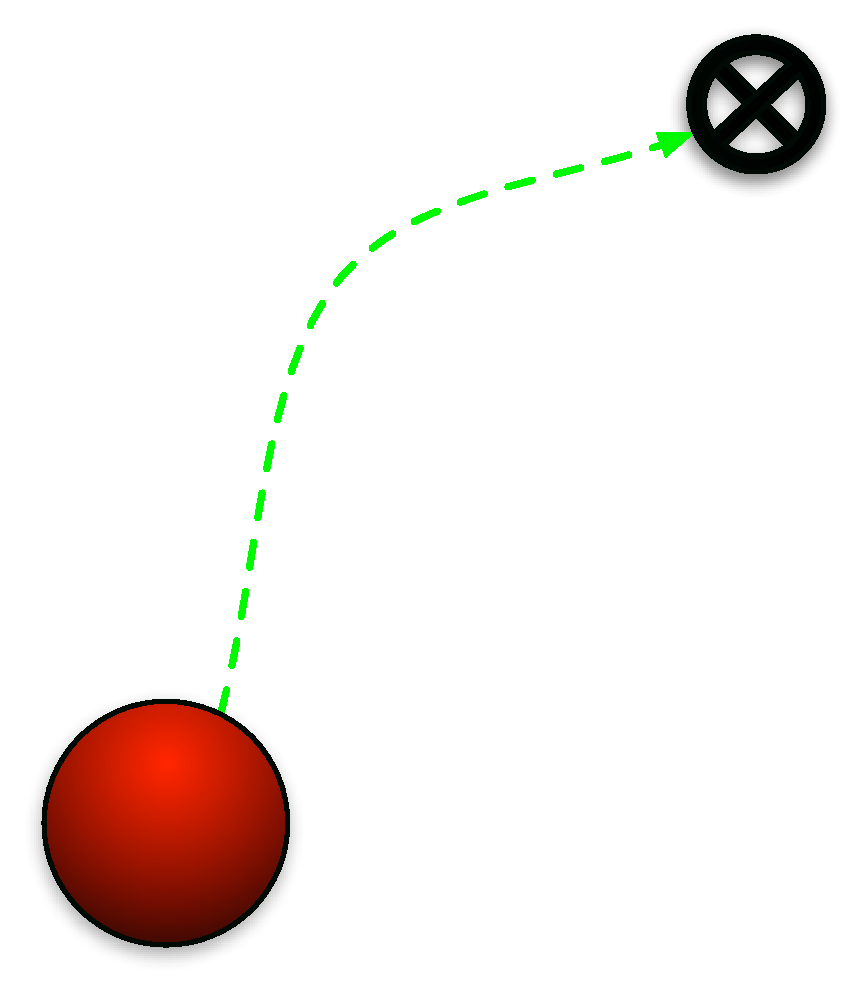
\includegraphics[scale=0.2]{../figures/seek.pdf}
			\caption{Seek and Pursuit}
			\end{center}
			\end{figure} 
		\end{column}
	
		\begin{column}{6cm}
			\pause
			\begin{figure}[htbp]
			\begin{center}
			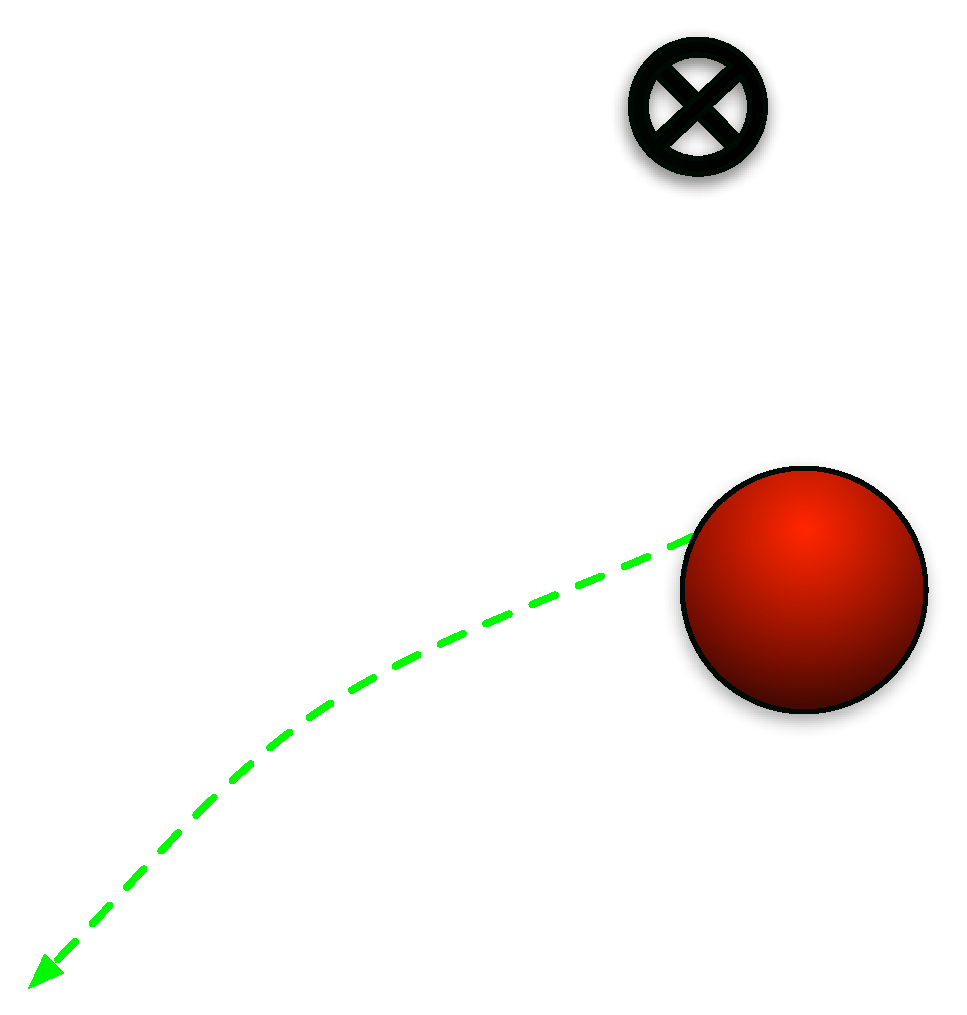
\includegraphics[scale=0.2]{../figures/avoid.pdf}
			\caption{Flee and Evasion}
			\end{center}
			\end{figure}
		\end{column}
	\end{columns}
\end{frame}
		
\begin{frame}{Previous Flocking Work}
	\begin{columns}[b]
		\begin{column}{6cm}
			\begin{figure}[htbp]
			\begin{center}
			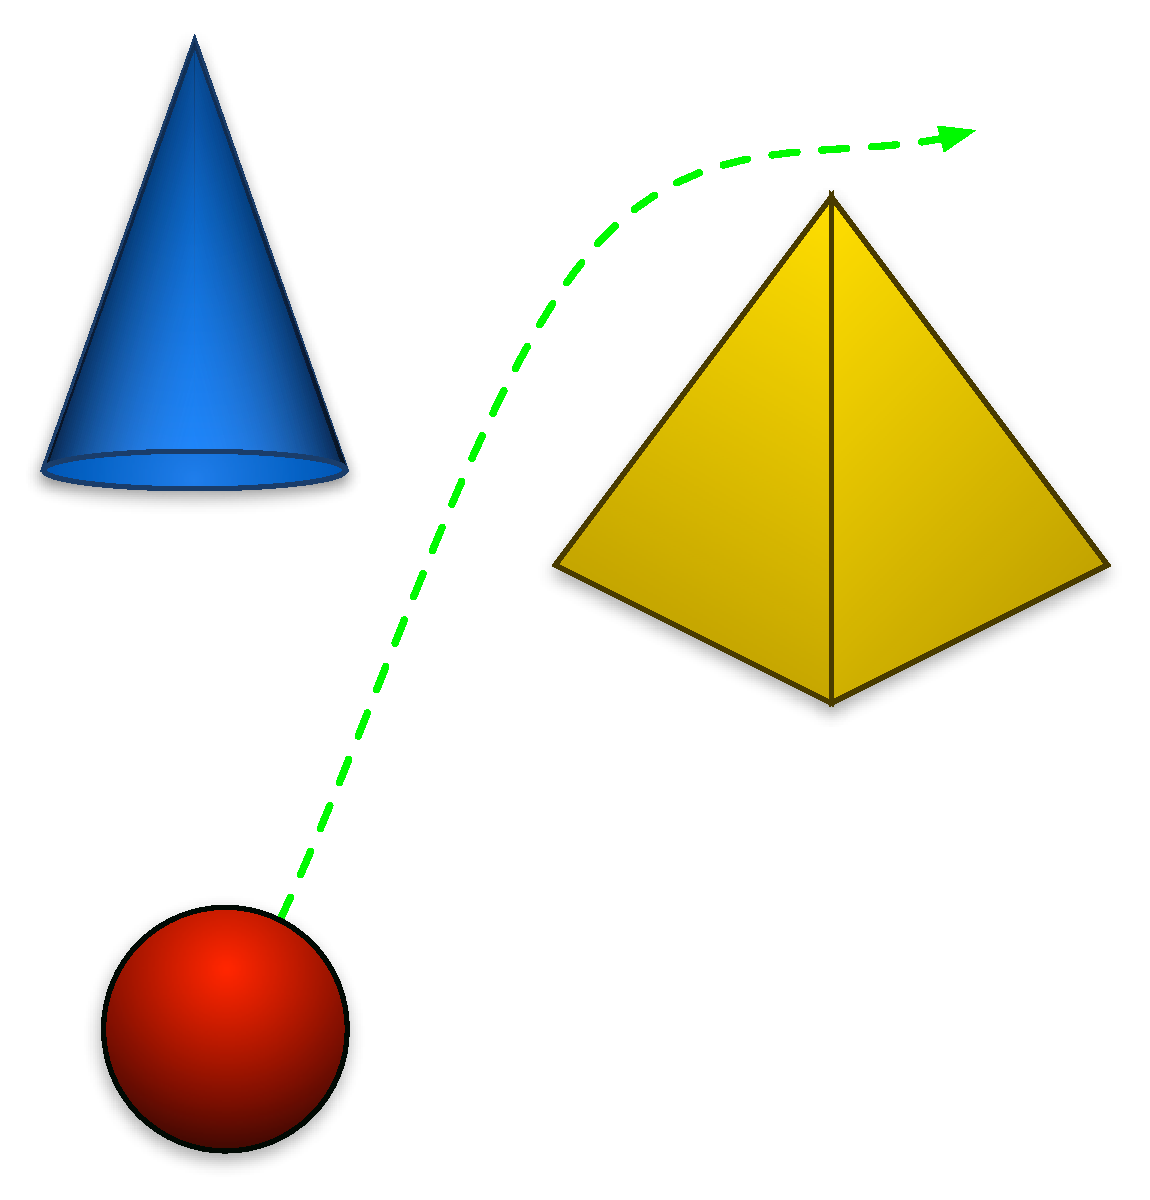
\includegraphics[scale=0.2]{../figures/obstacle.pdf}
			\caption{Obstacle Avoidance}
			\end{center}
			\end{figure} 
		\end{column}
	
		\begin{column}{6cm}
			\pause
			\begin{figure}[htbp]
			\begin{center}
			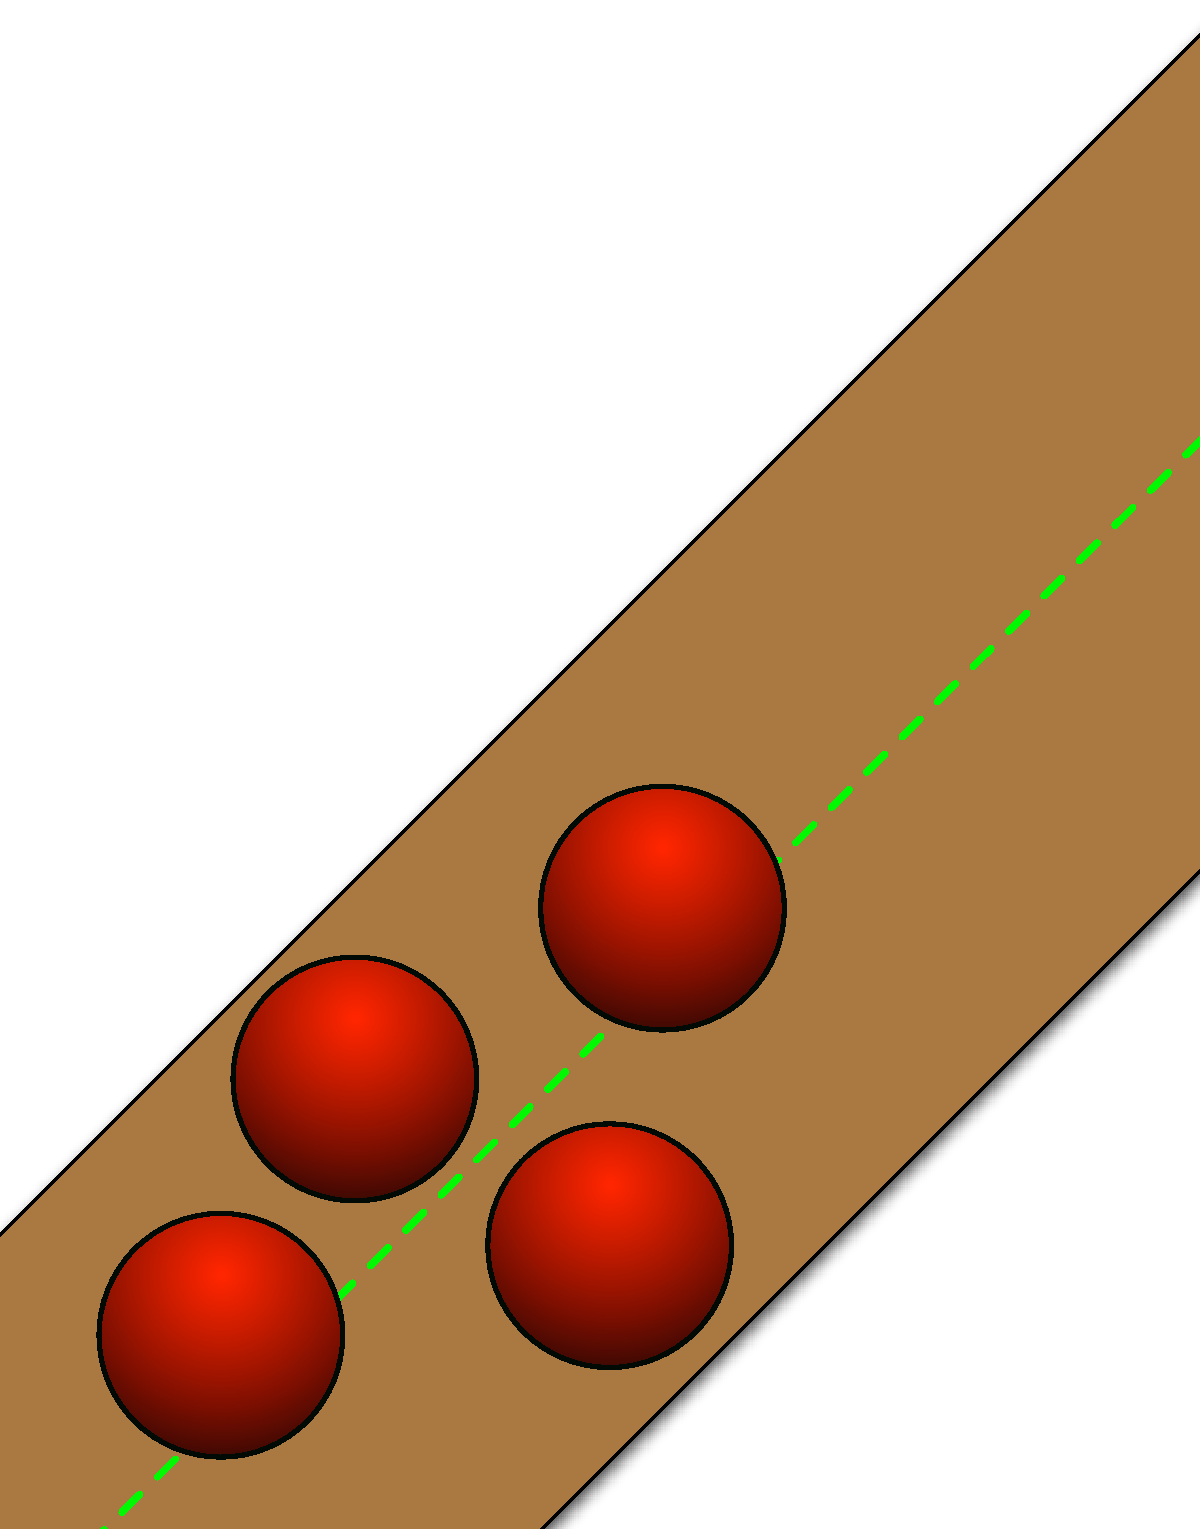
\includegraphics[scale=0.2]{../figures/pathFollowing.pdf}
			\caption{Path Following}
			\end{center}
			\end{figure}
		\end{column}
	\end{columns}
\end{frame}		
			
			
% applications
\begin{frame}{Applications}
	\pause Prey and predator simulations
	\begin{figure}[htbp]
	\begin{center}
	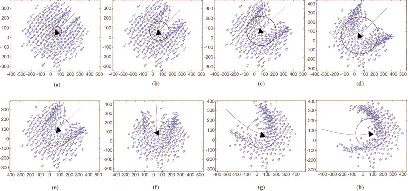
\includegraphics[scale=1.3]{figures/predatorPrey.pdf}
	\caption{\textit{Predator�s attack-induced phase-like transition in prey flock} by S.-H. Lee (2006)}
	\end{center}
	\end{figure}	
\end{frame}

\begin{frame}{Applications}		
 	Crowding simulations
	\begin{figure}[htbp]
	\begin{center}
	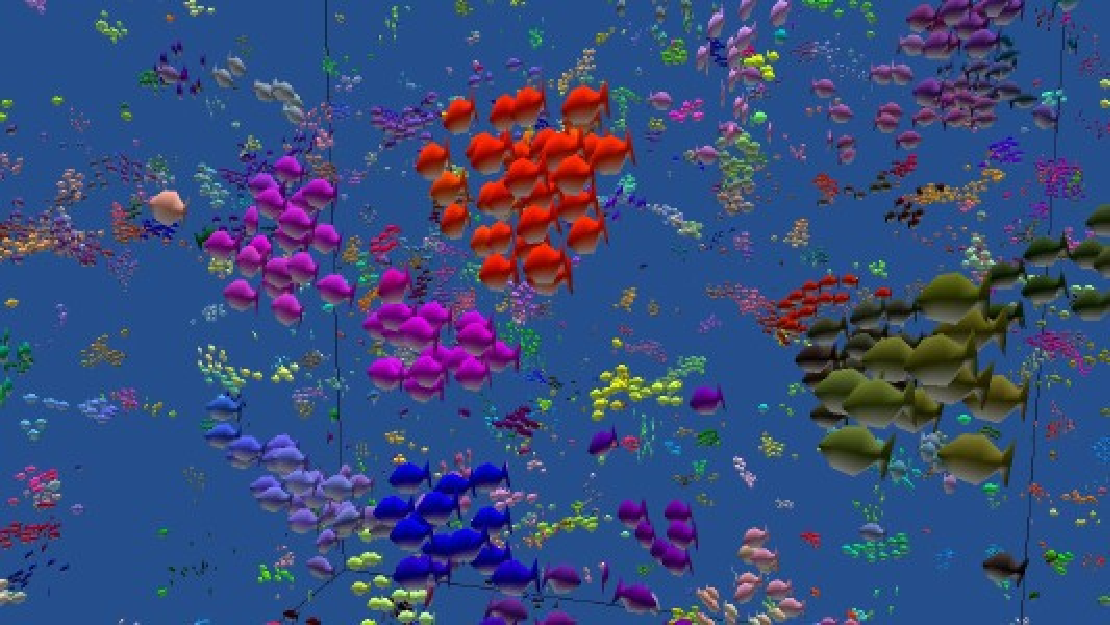
\includegraphics[scale=0.47]{figures/crowds.pdf}
	\caption{\textit{Big Fast Crowds on PS3} by Craig Reynolds (2006)}
	\end{center}
	\end{figure}
\end{frame}

\begin{frame}{Applications}	
	Robotics
	\begin{figure}[htbp]
	\begin{center}
	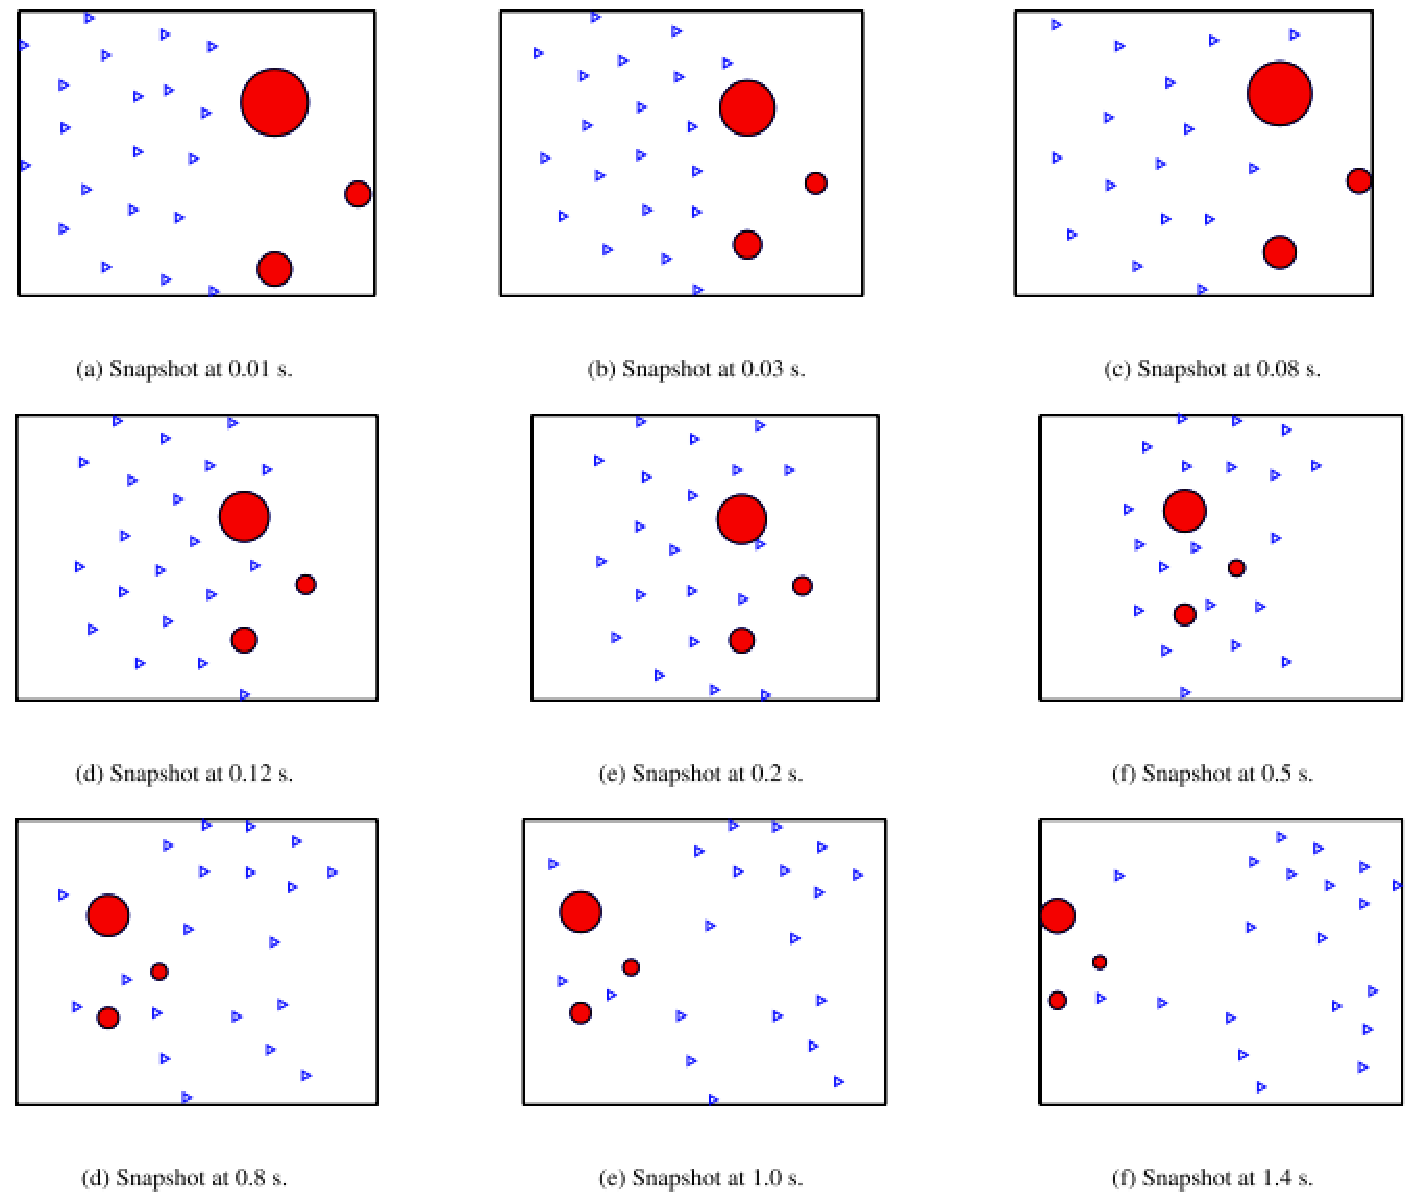
\includegraphics[scale=0.23]{figures/robots.pdf}
	\caption{\textit{A Decentralized and Adaptive Flocking Algorithm for Autonomous Mobile Robots} by Yan Yang et al. (2008) }
	\end{center}
	\end{figure}	
\end{frame}

\begin{frame}{Applications}
	Document clustering
	\begin{figure}[htbp]
	\begin{center}
	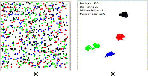
\includegraphics[scale=3.5]{figures/documents.pdf}
	\caption{\textit{A flocking based algorithm for document clustering analysis} by Xiaohui Cui et al. (2006)}
	\end{center}
	\end{figure}
\end{frame}

% GPU computing
\begin{frame}{GPU Computing}
	\begin{itemize}
		\pause \item Graphical processing units or \textit{GPUs} are numeric computing engines used to perform a massive number of floating-point calculations in parallel.
		\pause \item \textit{GPU computing}, also know as \textit{GPGPU} is a field of study that develops the use of GPUs for general purpose computing.
		\pause \item GPU computing is often considered an heterogeneous system, a mixture of GPUs and CPUs used together to process one or more tasks.
		\pause \item GPUs have different architecture than the CPUs therefore, special languages have been developed (e.g. CUDA, OpenCL). 
	\end{itemize}
\end{frame}

% flocking using the GPU
\begin{frame}{Flocking Using the GPU}
	\begin{itemize}
		\pause \item Flocking algorithms is amenable to massive parallelization since each boid is subject to identical rules.
		\pause \item Thus, the power of GPUs  can be leveraged to implement flocking strategies with upwards of tens or hundreds of thousands of boids.
	\end{itemize}
\end{frame}

%--------------------------------------------
% aim
%--------------------------------------------
\subsection{Aim}
\begin{frame}{Aim}
	\begin{itemize}
		\pause \item To develop a flocking implementation that can be used in the Blender Game Engine.
	\end{itemize}
\end{frame}

%--------------------------------------------
% flocking algorithm
%--------------------------------------------
\section{Rules and Algorithm}

\begin{frame}
	\begin{center}
		\textbf{Rules and Algorithm}
	\end{center}
\end{frame}

\begin{frame}{Flocking}
	\begin{itemize}
		\pause \item \textit{Flocking} is used to simulate social behavior between entities by following a simple set of rules.
		\pause \item The three main rules, also called \textit{steering behaviors} are:
			\begin{itemize}
				\pause \item Separation
				\pause \item Alignment
				\pause \item Cohesion
			\end{itemize}
		\pause \item Each rule is associated with a velocity vector and a scalar weight.
	\end{itemize}
\end{frame}

%--------------------------------------------
% 3 behaviors
%--------------------------------------------
\subsection{Three Main Steering Behaviors}

% separation
\begin{frame}{Separation}
	% equation: separation 
	\begin{equation}
	\label{separationEquation}
	Separation =\frac{1}{M} \sum_{n=1}^{M} \frac{p_i - p_n}{d(p_i,p_n)}
	\end{equation}
	
	% figure: separation
	\begin{figure}[htbp]
	\begin{center}
	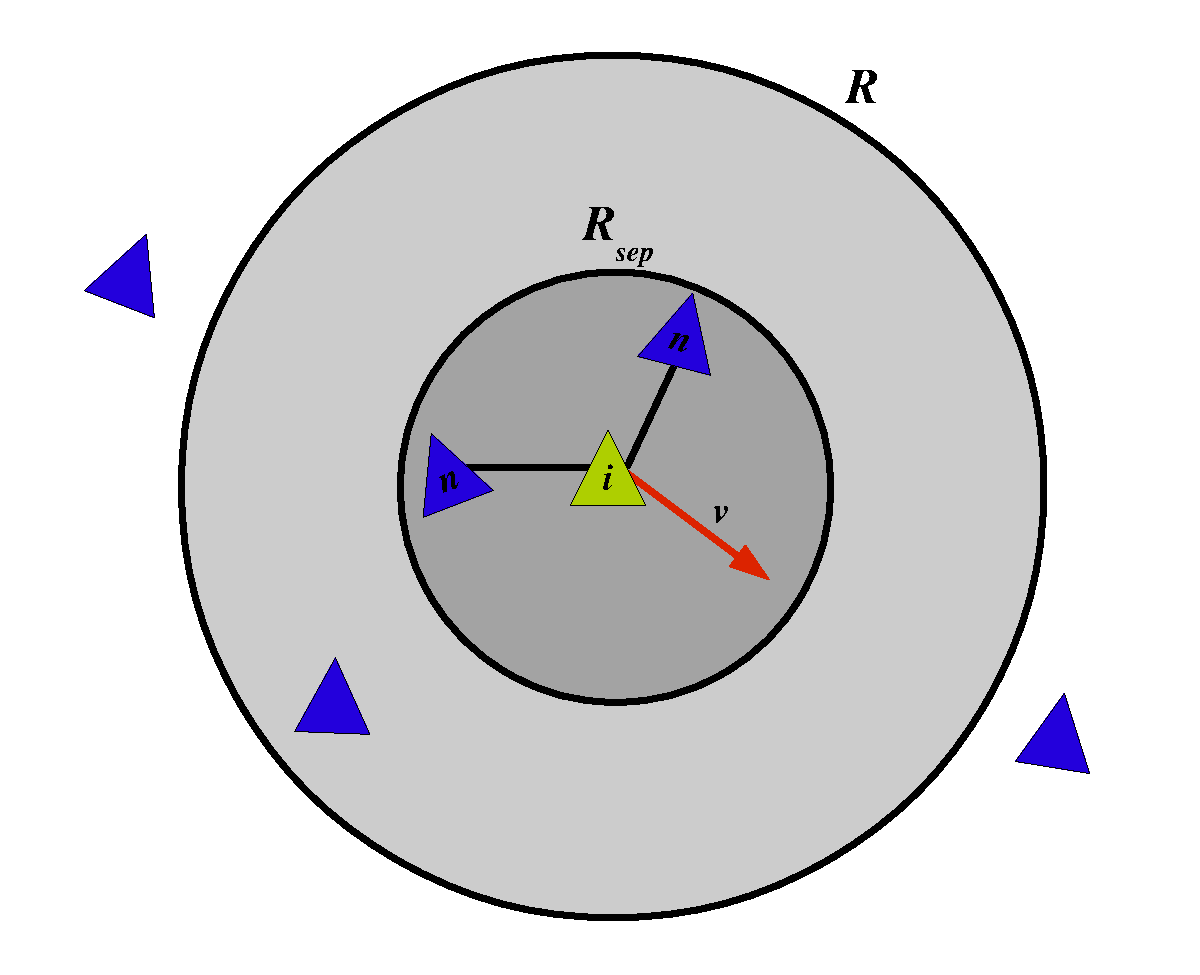
\includegraphics[scale=0.45]{../figures/separation.pdf}
	%\caption{Separation steering behavior}
	\label{separation}
	\end{center}
	\end{figure}
\end{frame}

% alignment
\begin{frame}{Alignment}
	% equation: alignment
	\begin{equation}
	\label{alignmentEquation}
	Alignment = \left[  \frac{1}{N} \sum_{n=1}^{N} v_n \right ] - v_i
	\end{equation}
	
	% figure: alignment
	\begin{figure}[htbp]
	\begin{center}
	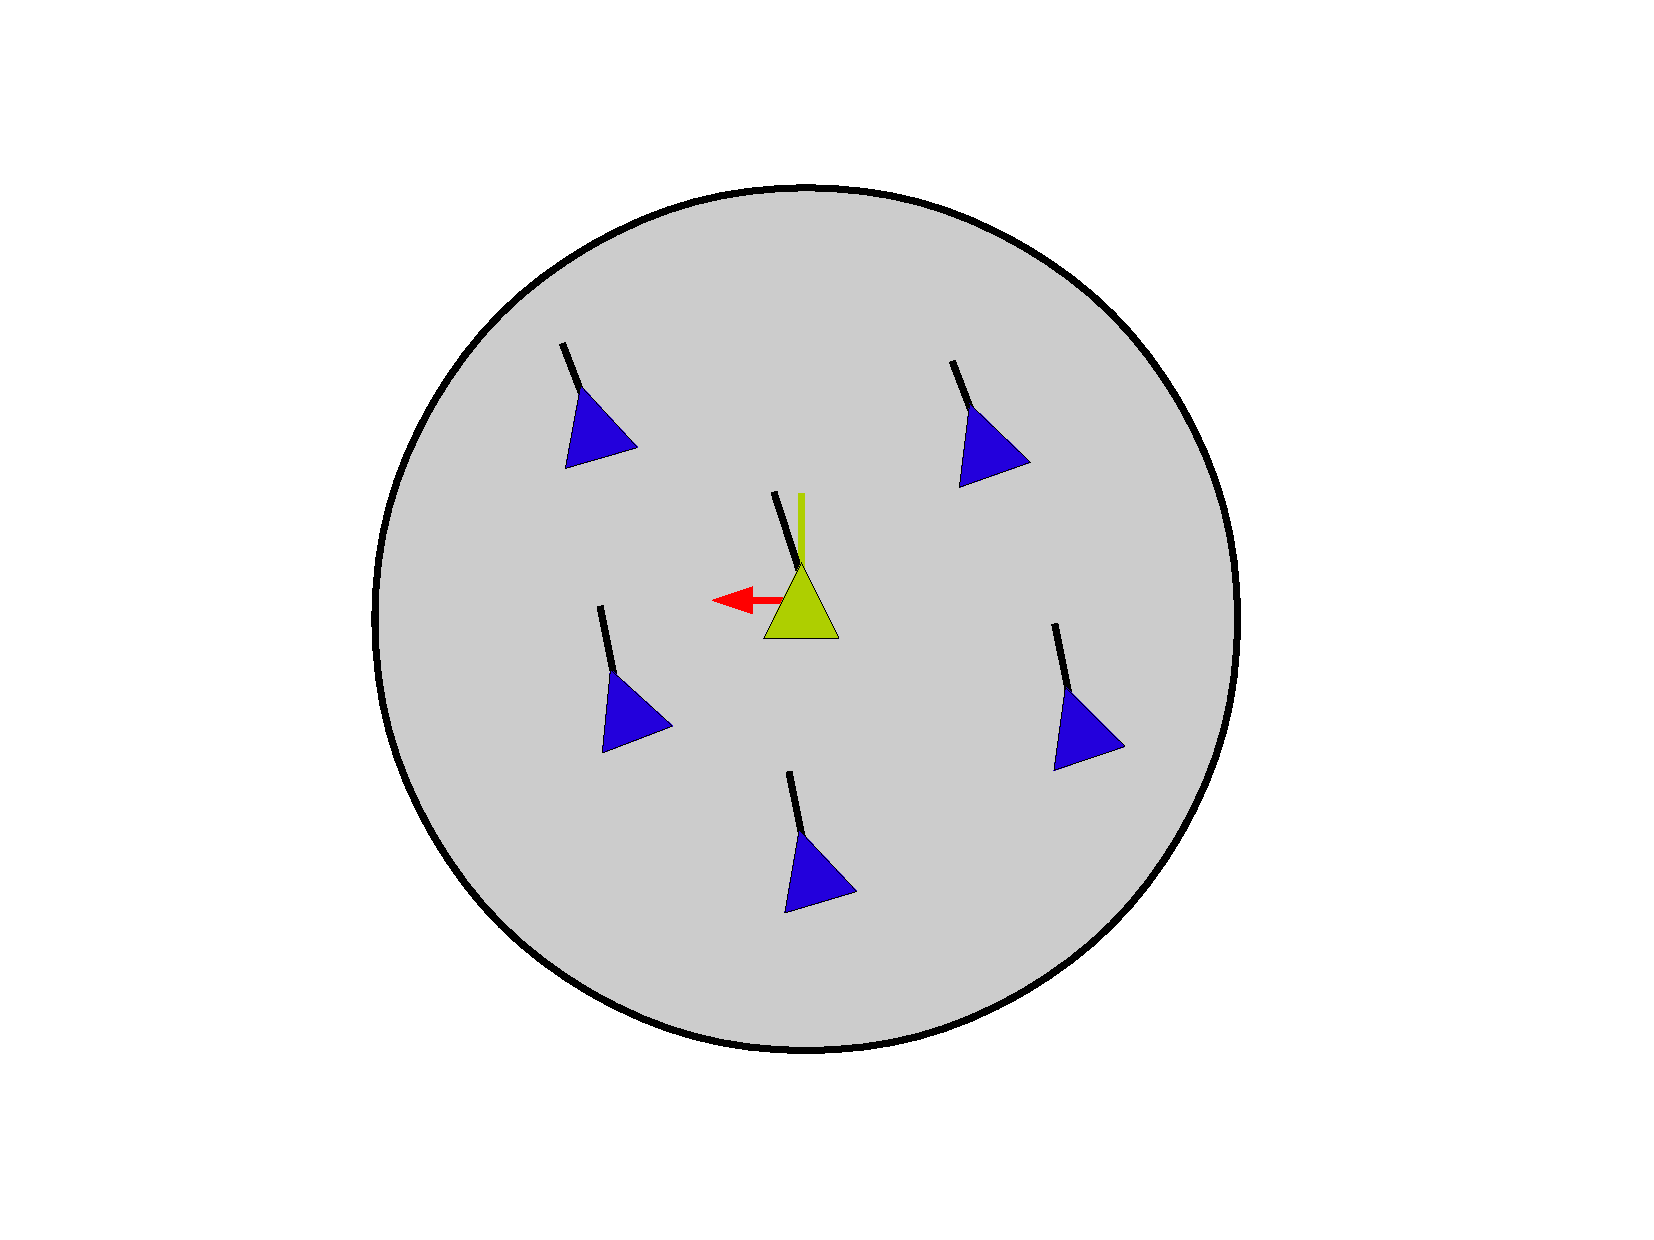
\includegraphics[scale=0.45]{../figures/alignment.pdf}
	%\caption{Alignment steering behavior}
	\label{alignment}
	\end{center}
	\end{figure}
\end{frame}

% cohesion
\begin{frame}{Cohesion}
	% equation: cohesion
	\begin{equation}
	\label{cohesionEquation}
	Cohesion = \left[  \frac{1}{N} \sum_{n=1}^{N} p_n \right ] - p_i
	\end{equation}
	
	% figure: cohesion
	\begin{figure}[htbp]
	\begin{center}
	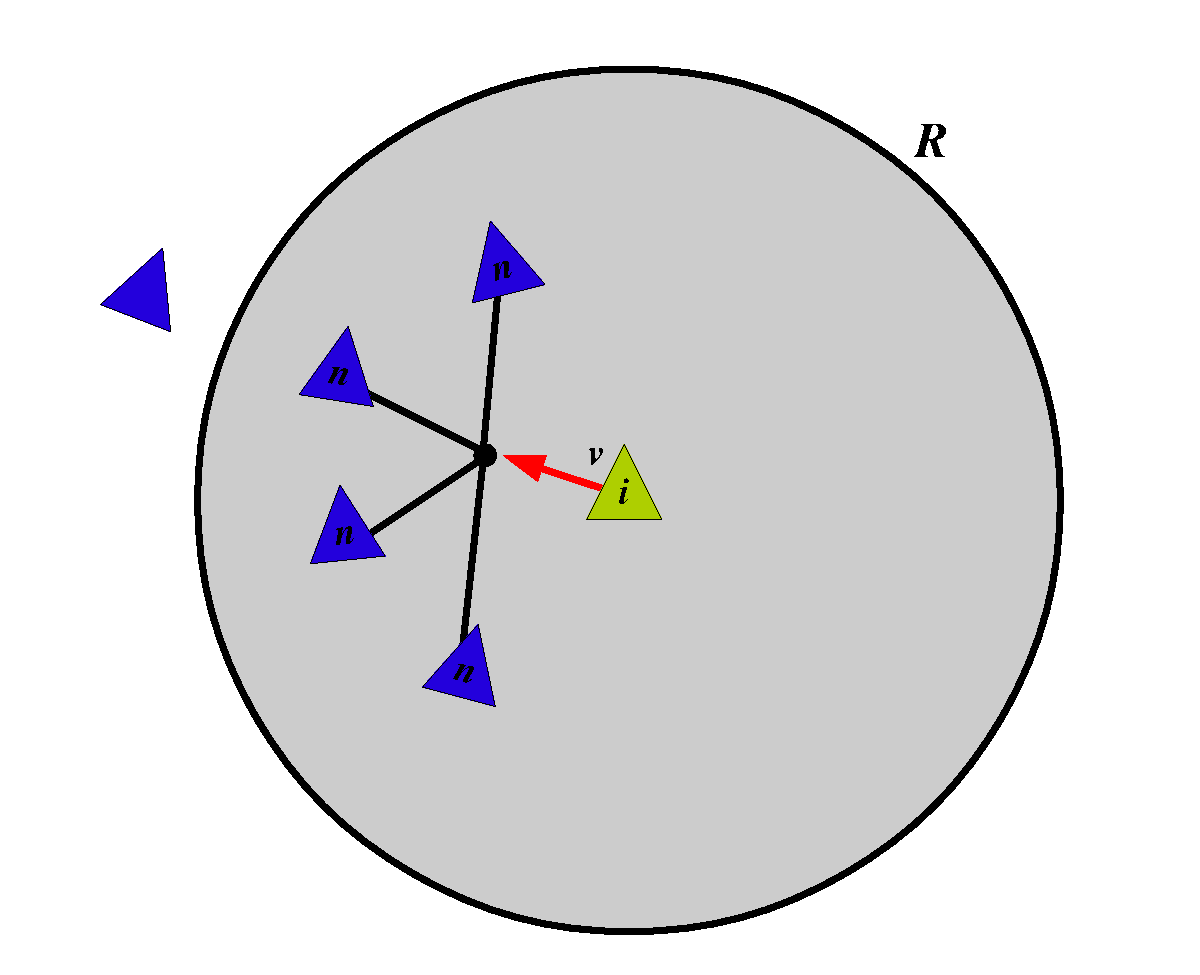
\includegraphics[scale=0.45]{../figures/cohesion.pdf}
	%\caption{Cohesion steering behavior}
	\label{cohesion}
	\end{center}
	\end{figure}
\end{frame}

%--------------------------------------------
% other behaviors
%--------------------------------------------
\subsection{Other Steering Behaviors}

% goal 
\begin{frame}{Goal}
	% goal equation
	\begin{equation}
	\label{goalEquation}
	Goal = \left(\frac{p_t - p_i}{d(p_t,p_i)} * max_{speed}\right) - v_i
	\end{equation}
	
	% figure: seek and flee
	\begin{figure}[htbp]
	\begin{center}
	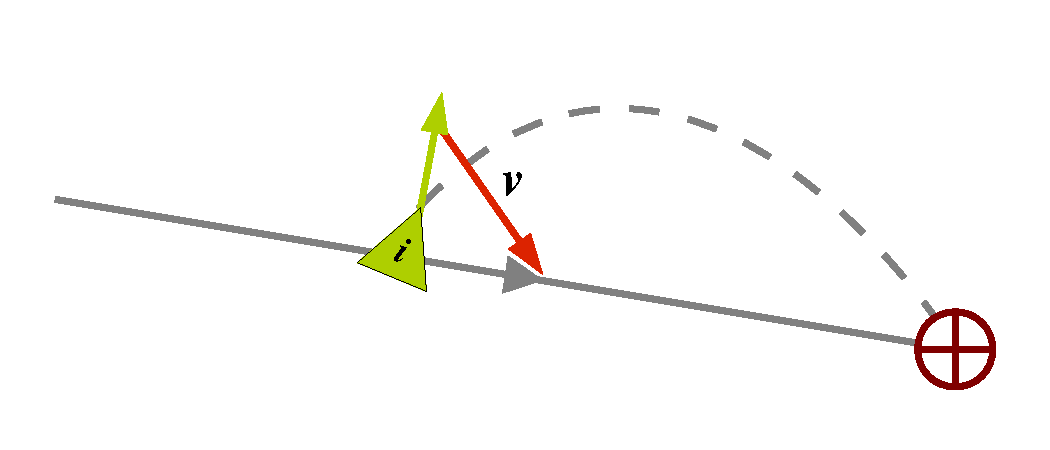
\includegraphics[scale=0.65]{../figures/goal.pdf}
	%\caption{Goal steering behavior}
	\label{seekANDflee}
	\end{center}
	\end{figure}
\end{frame}

% avoid
\begin{frame}{Avoidance}
	\begin{equation}
	\label{avoidEquation}
	Avoidance = -\left(\frac{p_t - p_i}{d(p_t,p_i)} * max_{speed}\right) - v_i
	\end{equation}

	% figure: seek and flee
	\begin{figure}[htbp]
	\begin{center}
	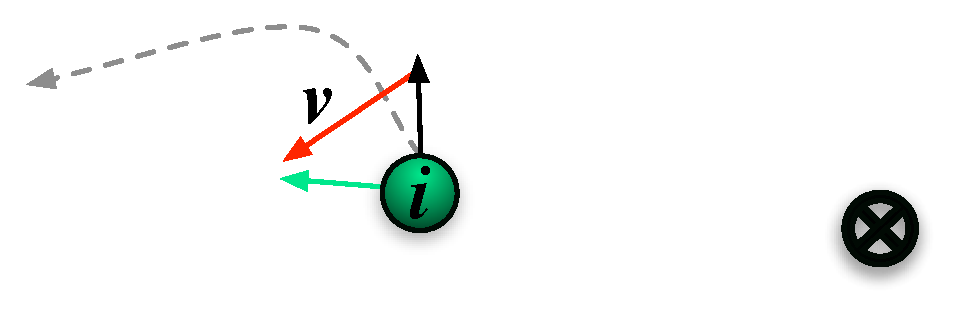
\includegraphics[scale=0.65]{../figures/avoidance.pdf}
	%\caption{Avoidance steering behavior}
	\label{seekANDflee}
	\end{center}
	\end{figure}
\end{frame}
% avoid equation
	
% combine
\begin{frame}{Final Velocity}
	The final velocity of the boids is calculated as a linear combination of the steering behaviors.
	 
	\begin{equation}
	vel^{k+1} = vel^{k} + \sum_{rule_r} w_{rule_r} {rule_r}
	\end{equation}
	
	where ${rule}_r$ is the resulting velocity of each steering behavior and $w_{rule_r}$ is the respective scalar weight for that rule. 
	 
\end{frame}

%--------------------------------------------
% algorithm
%--------------------------------------------
\subsection{Flocking Algorithm}

% rules
\begin{frame}{Compute the Rules}
	\alert<1>{$for$ each boid $i$ $do$}	 \\
	\alert<2>{~~$for$ each neighbor $j$ of boid $i$ $do$}			\\
	\alert<3>{~~~~$if$ d($pos_i$, $pos_j$) $<=$ searching radius $then$}	\\
	\alert<4>{~~~~~~$if$ $w_{rule_r}$ $>$ 0 $then$}					\\
	\alert<4>{~~~~~~~~~~Compute $rule_r$}  \\
	\alert<4>{~~~~~~end $if$} \\
	\alert<5>{~~~~~~$Comment: Compute ~all ~the ~other ~rules. $} \\
	\alert<3>{~~~~end $if$} \\
	\alert<2>{~~end $for$} \\
	\alert<1>{end $for$}
\end{frame}

% integration
\begin{frame}{Combine and Integrate}
	\alert<1>{$vel_i^{k+1} = vel_i^{k} + \sum_{rule_r} w_{rule_r} {rule_r}$} 	\\ 
	\alert<2>{$if$ length($vel_i^{k+1}$) $>$ $max_{speed}$ $then$}			\\ 
	\alert<2>{~~$vel_i^{k+1}$ = normalize($vel_i^{k+1}$)  $max_{speed}$} \\
	\alert<2>{end $if$} \\
	\alert<3>{(Optional) Add an imposed velocity to the current velocity.}	\\ 
	\alert<4>{$pos_i^{k+1}$ = $pos_i^{k}$  + $dt $ $vel_i^{k+1}$}					\\
	\alert<5>{Apply periodic boundary conditions to the \textit{new} position.} 
\end{frame}


%--------------------------------------------
% implementation
%--------------------------------------------
\section{Implementation}

\begin{frame}
	\begin{center}
		\textbf{Implementation}
	\end{center}
\end{frame}

%--------------------------------------------
% RTPS
%--------------------------------------------
\subsection{The RTPS Library}

% RTPS diagram
\begin{frame}{RTPS organization diagram}
	\pause
	\begin{figure}[htbp]
	\begin{center}
	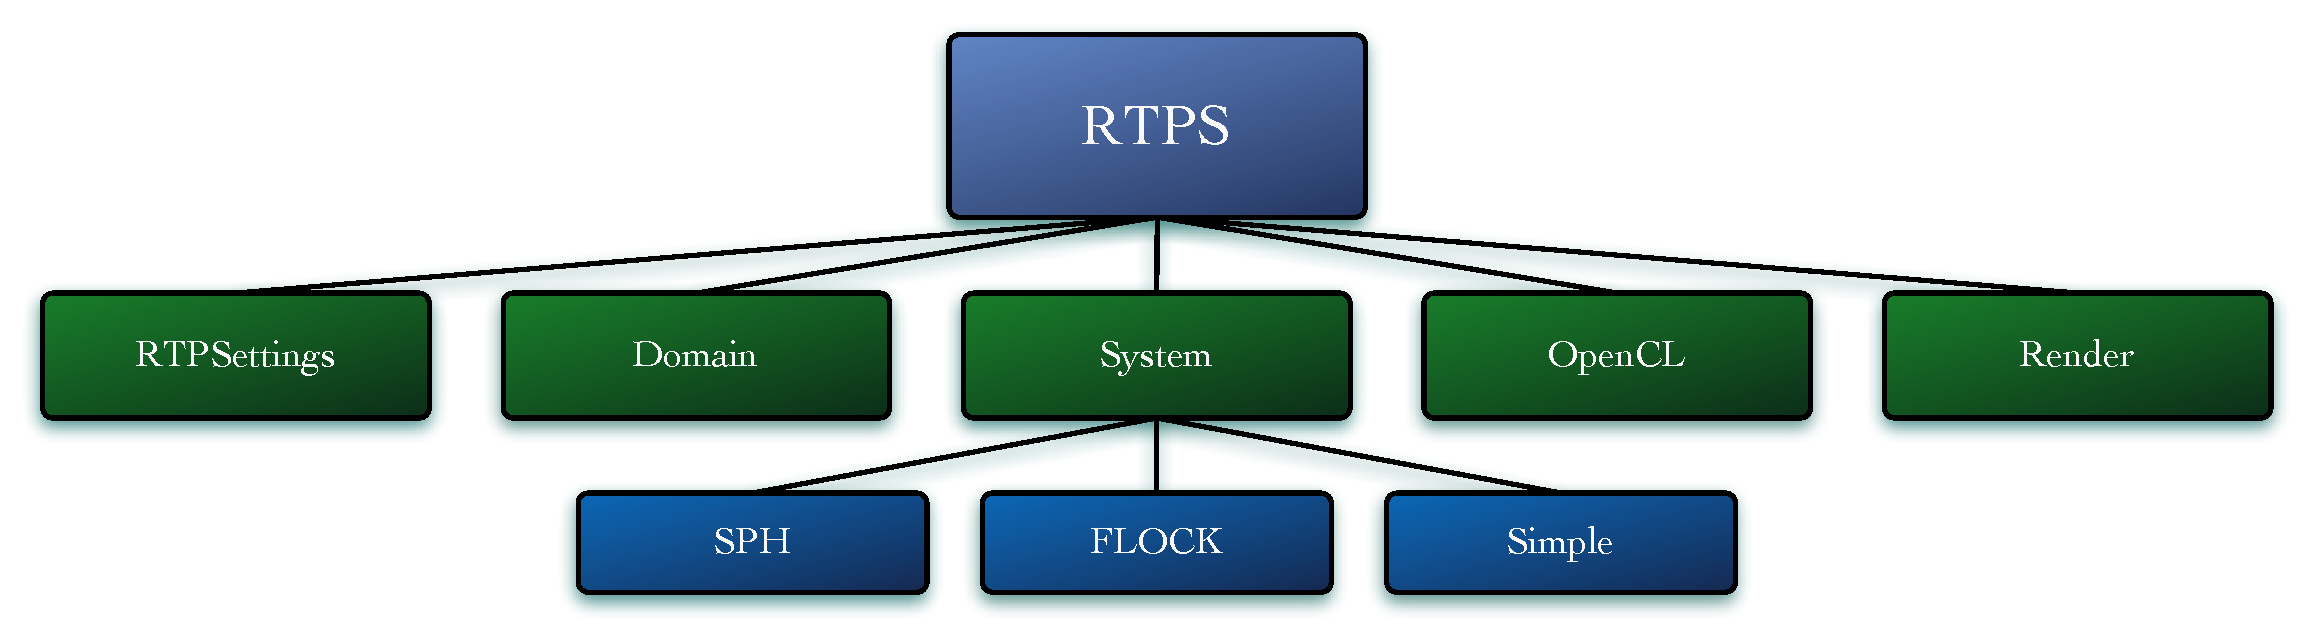
\includegraphics[scale=0.28]{../figures/RTPSdiagramMyrna.pdf}
	%\caption{RTPS organization diagram}
	\end{center}
	\end{figure}
\end{frame}

% FLOCK diagram
\begin{frame}{FLOCK system organization diagram}
	\pause
	\begin{figure}[htbp]
	\begin{center}
	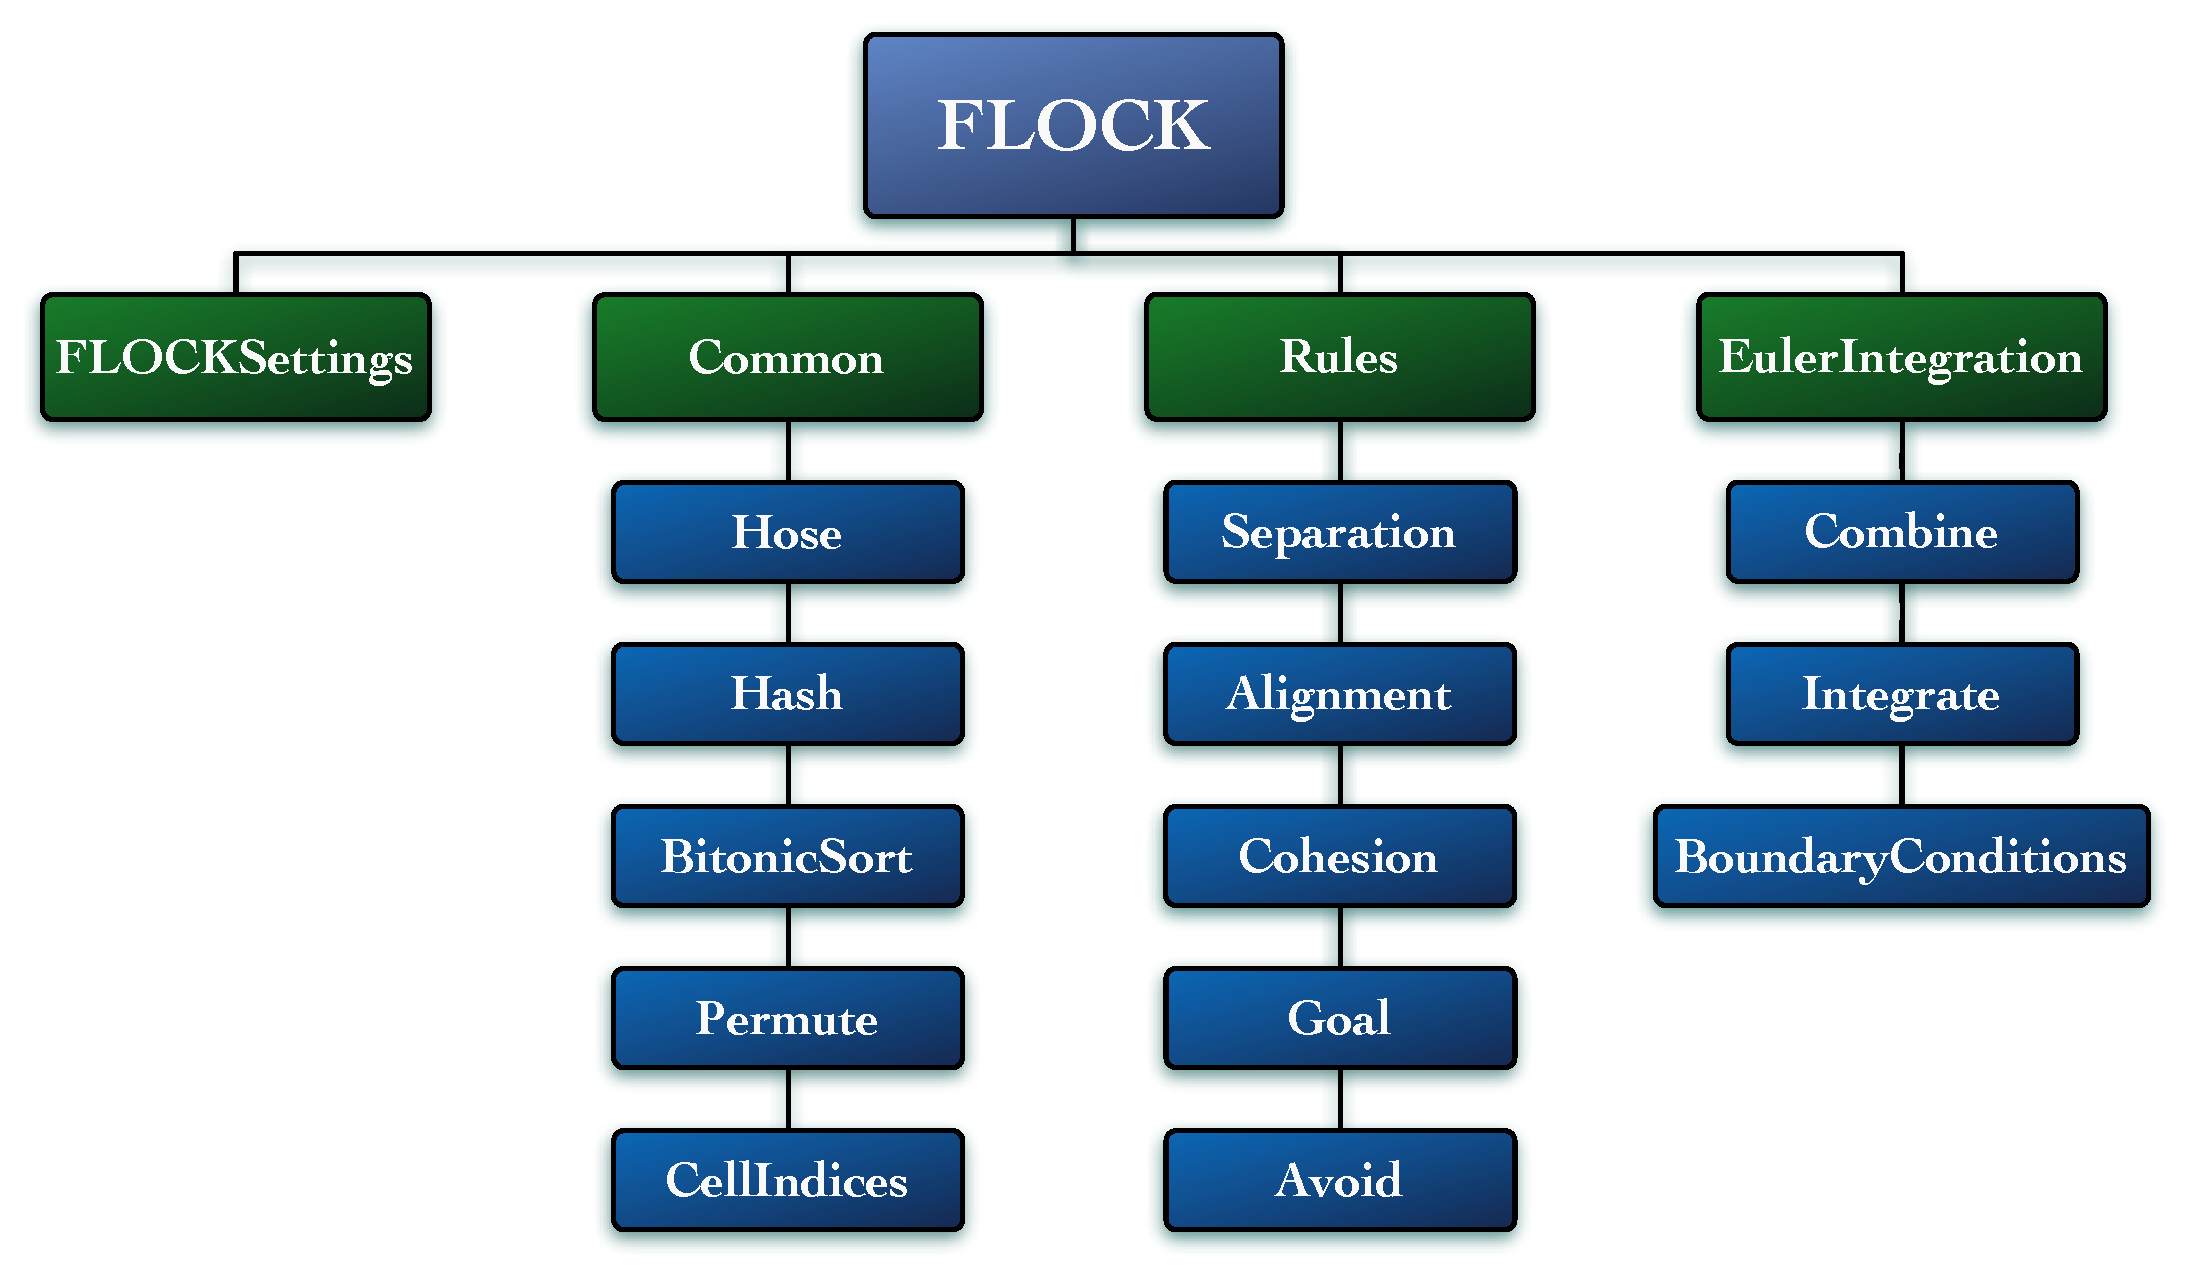
\includegraphics[scale=0.25]{../figures/FLOCKdiagramMyrna.pdf}
	%\caption{FLOCK system organization diagram}
	\end{center}
	\end{figure}
\end{frame}

% NNS
\begin{frame}{Nearest Neighbor Search}
	%\pause Two phases: \textit{preparation} and \textit{lookup}.
	
	\pause
	\begin{figure}[htbp]
	\begin{center}
	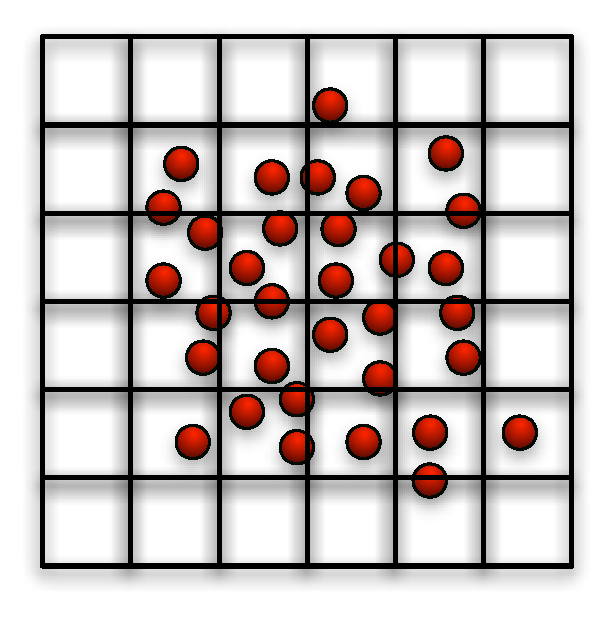
\includegraphics[scale=0.35]{../figures/hash.pdf}
	\caption{First step of NNS: Hash}
	\end{center}
	\end{figure}
	
	%\begin{cppcode}{0}
	$cell_{index} = ( pos - grid_{min} )  grid_{delta} $
	$hash = ( cell_{index_z} cells_y + cell_{index_y} )  cells_x + cell_{index_x}$
	%\end{cppcode}
	
\end{frame}

\begin{frame}{Nearest Neighbor Search}
	\begin{itemize}
		\pause \item \textbf{BitonicSort} sorts their hash array by the hash values
		\pause \item \textbf{Permute} permutes the arrays of positions, velocities and colors according to the sorted index array
		\pause \item \textbf{CellIndices} updates two arrays that keep track of the first and last boid at each cell
	\end{itemize}
\end{frame}

% FLOCK diagram
\begin{frame}{FLOCK system organization diagram}
	\begin{figure}[htbp]
	\begin{center}
	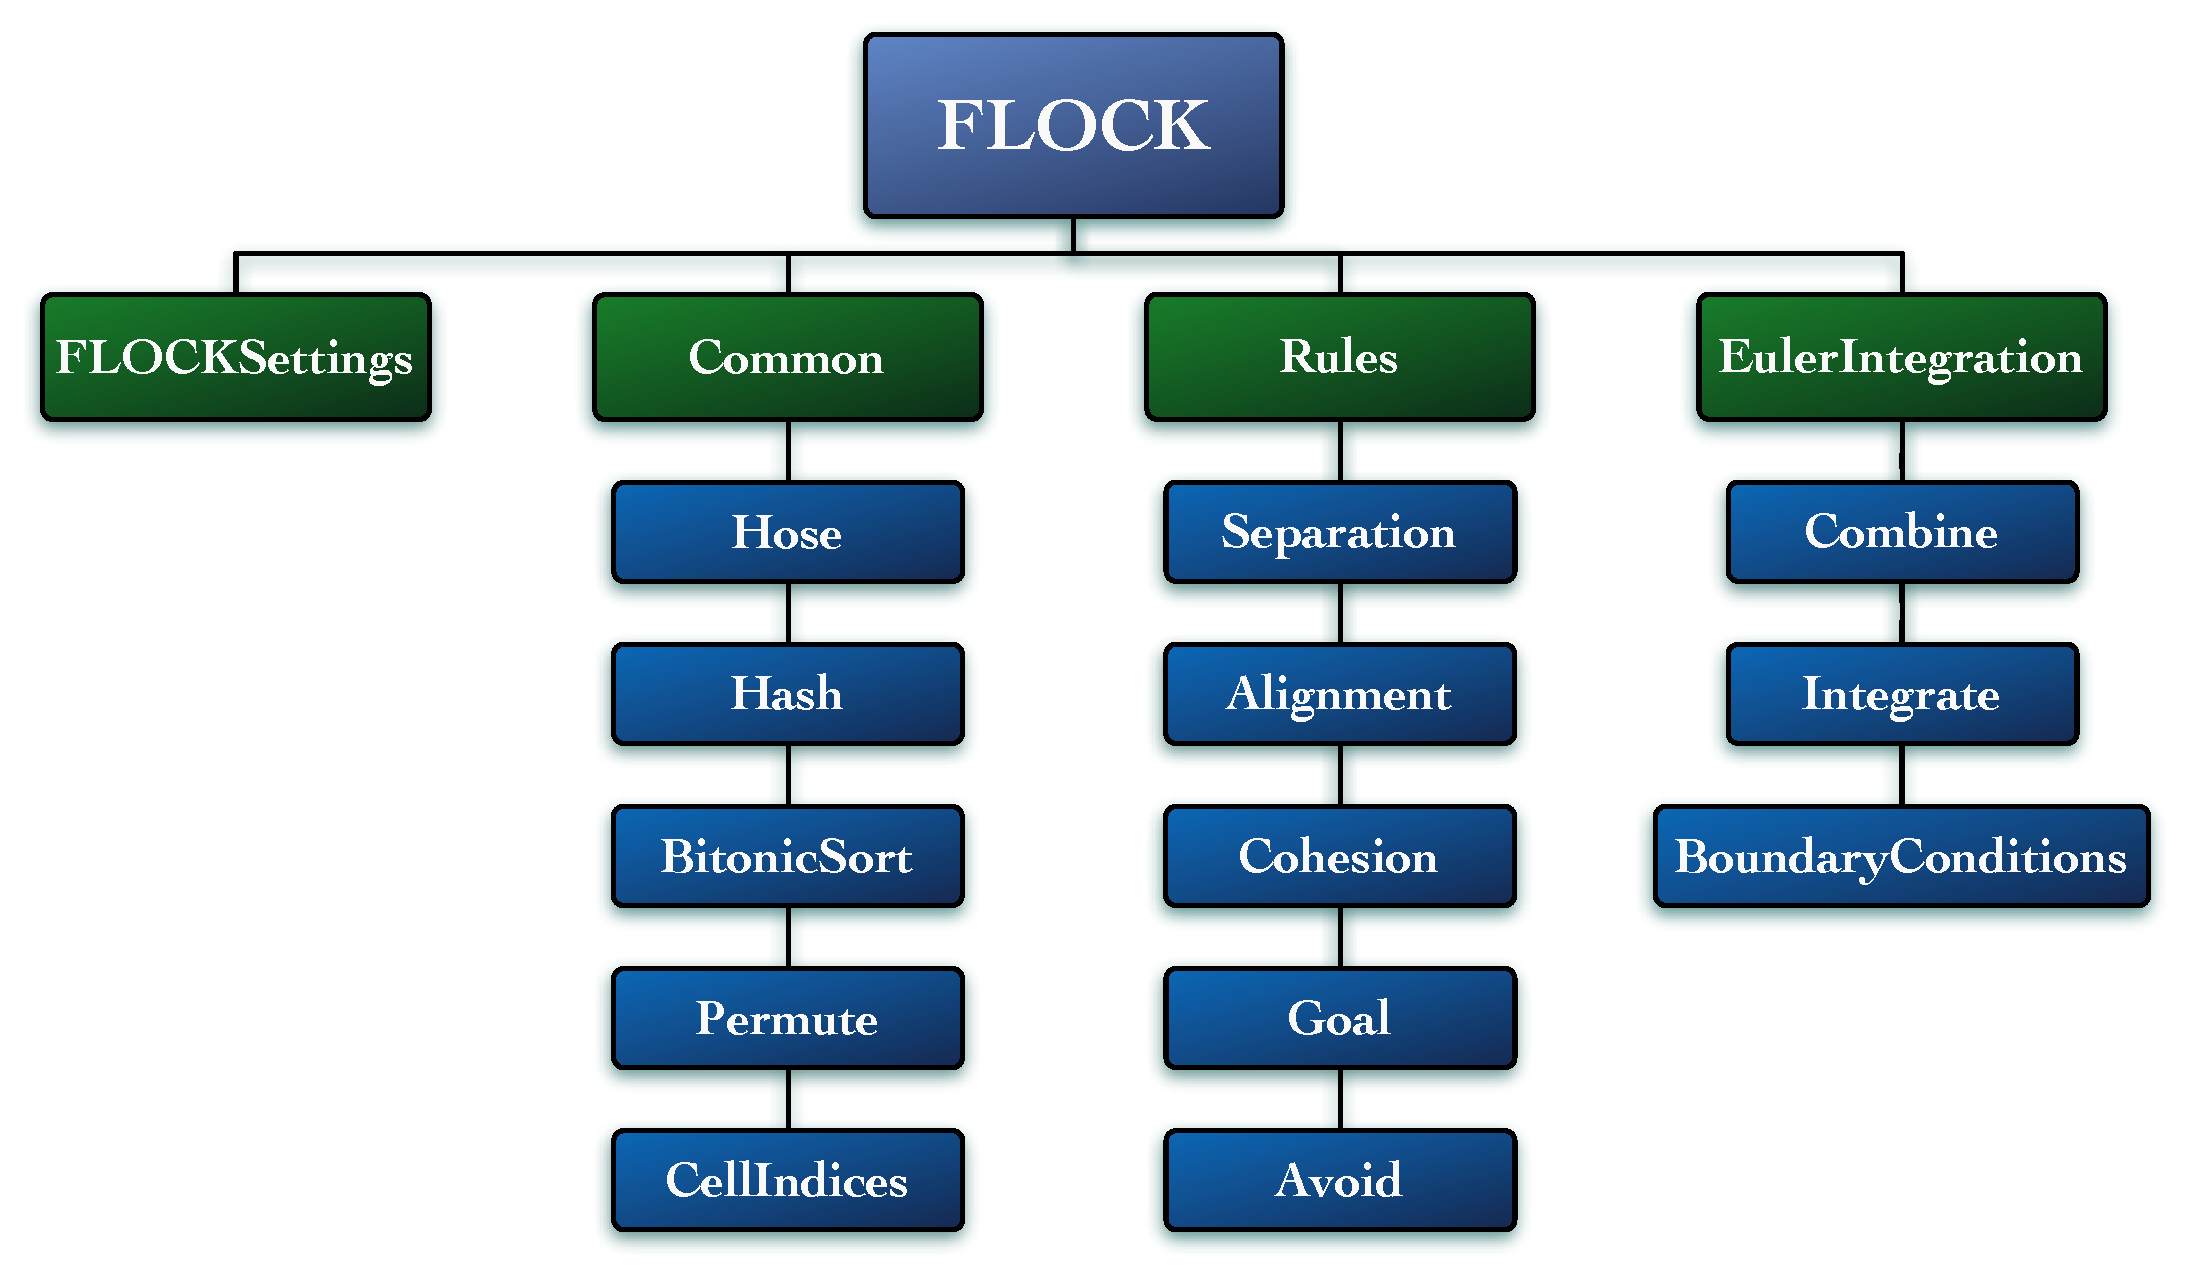
\includegraphics[scale=0.25]{../figures/FLOCKdiagramMyrna.pdf}
	%\caption{FLOCK system organization diagram}
	\end{center}
	\end{figure}
\end{frame}

%--------------------------------------------
% blender
%--------------------------------------------
\subsection{The RTPS Modifier}

% Blender
\begin{frame}{Blender}
	\begin{itemize}
		\pause \item Free 
		\pause \item Built-in game engine 
		\pause \item Powerful modeling/simulation tools
		\pause \item Open-source
		\pause \item Cross-platform
		\pause \item Has a strong and active community
	\end{itemize}
	\pause \em{Blender 2.57 was the release used in this project}.
\end{frame}

%--------------------------------------------
% BGE
%--------------------------------------------
\begin{frame}{The Blender Game Engine}
	\begin{itemize}
		\pause \item Game Engines are used to simulate virtual reality.
		\pause \item Let you interact with 3D world in real-time. \pause FUN!
		\pause \item The Blender Game Engine lets you create simple games can be created without the need for explicit programming.
		\pause \item After creating the 3D scene you can bring it to life by using the logic editor.	
	\end{itemize}
\end{frame}

\begin{frame}{The Blender Game Engine}
	% figure: logic editor 
	\pause
	\begin{figure}[htbp]
	\begin{center}
	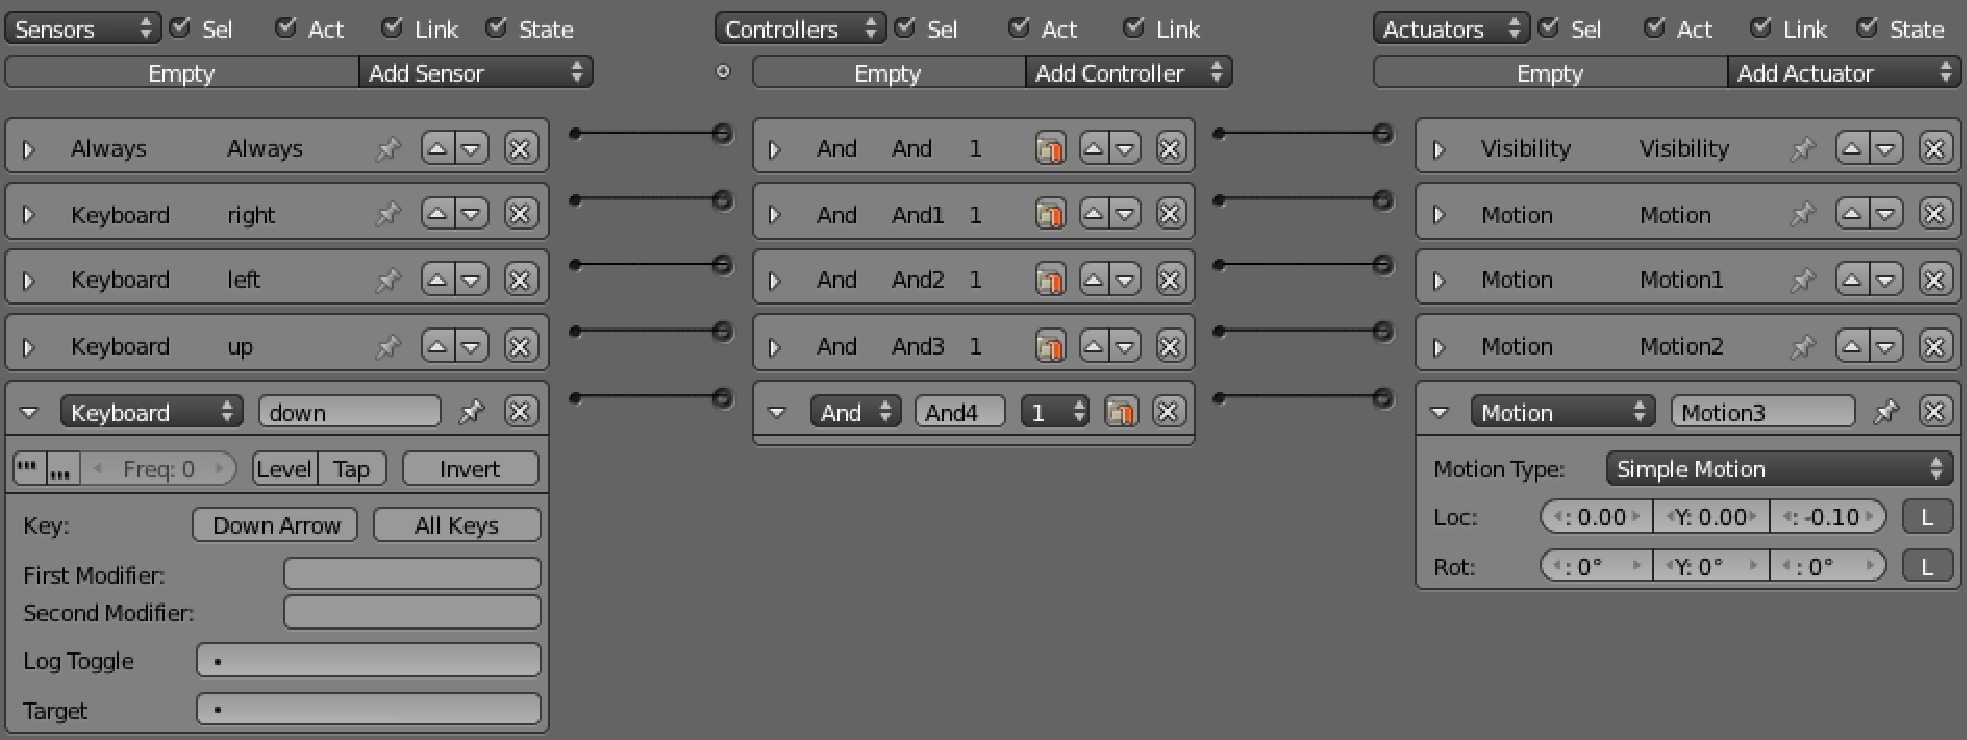
\includegraphics[scale=0.32]{../figures/logic_bricks.pdf}
	\end{center}
	\caption{Blender Game Logic Editor: Logic Bricks}
	\label{logicEditor}
	\end{figure}
\end{frame}

% The Blender Game Engine
\begin{frame}{The Blender Game Engine}
	\begin{itemize}
		\pause \item The Blender Game Engine has no particles systems.
		\pause \item We would like to add this missing feature to it.
		\pause \item A \textit{Boids} system is added to the Blender Game Engine as a modifier interface.
	\end{itemize}
\end{frame}

% The RTPS Modifier
\begin{frame}{The RTPS Modifier}
	\begin{figure}[htbp]
	\begin{center}
	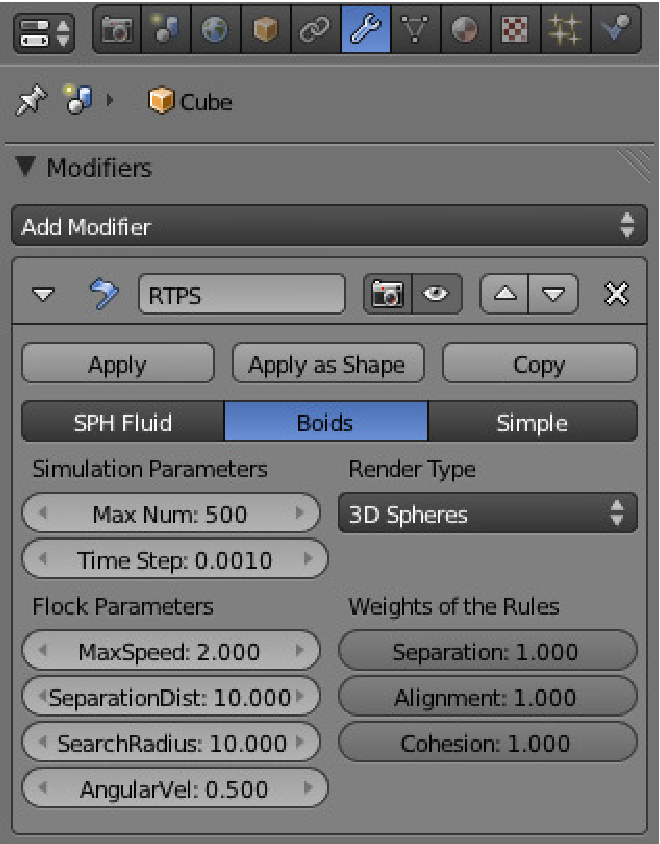
\includegraphics[scale=0.4]{../figures/modifier.pdf}
	%\caption{The RTPS modifier in the Boids system}
	\end{center}
	\end{figure}
\end{frame}

\begin{frame}{Emitting boids to the system}

	\begin{columns}
	
	\begin{column}{5cm}
	\begin{table}[htdp]
	%\caption{Properties available in the RTPS modifer}
	\begin{center}
	\begin{tabular}{|p{1.5cm}|p{3cm}|}
	\hline 
	\textbf{Property} & \textbf{Description} \\\hline 
	\texttt{num} 	& num boids are emitted and num is reset to 0	\\\hline 
	\texttt{hose}	& used to active the hose	\\\hline
	\texttt{speed}	& initial velocity of the boids emitted from the hose	\\\hline
	\texttt{radius}	& hose's width	\\
	\hline 
	\end{tabular}
	\end{center}
	\end{table}
	\end{column}
	
	\begin{column}{5cm}
	\begin{figure}[htbp]
	\begin{center}
	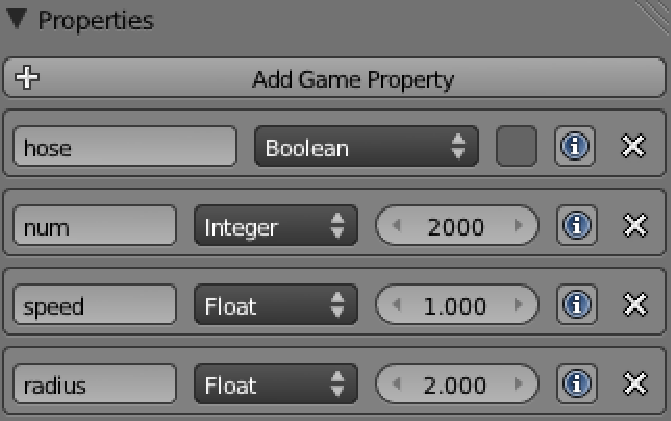
\includegraphics[scale=0.45]{../figures/logic_properties.pdf}
	\end{center}
	\caption{Blender Properties}
	\label{logicEditor}
	\end{figure}
	\end{column}
	
	\end{columns}
\end{frame}


%--------------------------------------------
% results
%--------------------------------------------
\section{Results}

\begin{frame}
	\begin{center}
		\textbf{Results}
	\end{center}
\end{frame}

%--------------------------------------------
% timings
%--------------------------------------------
\subsection{Benchmarks}

% RTPS vs RTPS
\begin{frame}{RTPS-FLOCK system}

	\begin{columns}
	\begin{column}{2.25cm}
	\scriptsize
	~\textbf{Settings} \\
	~~maxBoids=256K \\
	~~maxSpeed = 2 \\
	~~searchRad = 1.5 \\
	~~minDist = 1 \\
	~~w\_sep = 1 \\
	~~w\_align = 1 \\
	~~w\_coh = 1 \\
	~~w\_goal = 0 \\
	~~w\_avoid = 0 \\
	\end{column}
	
	\begin{column}{15cm}
	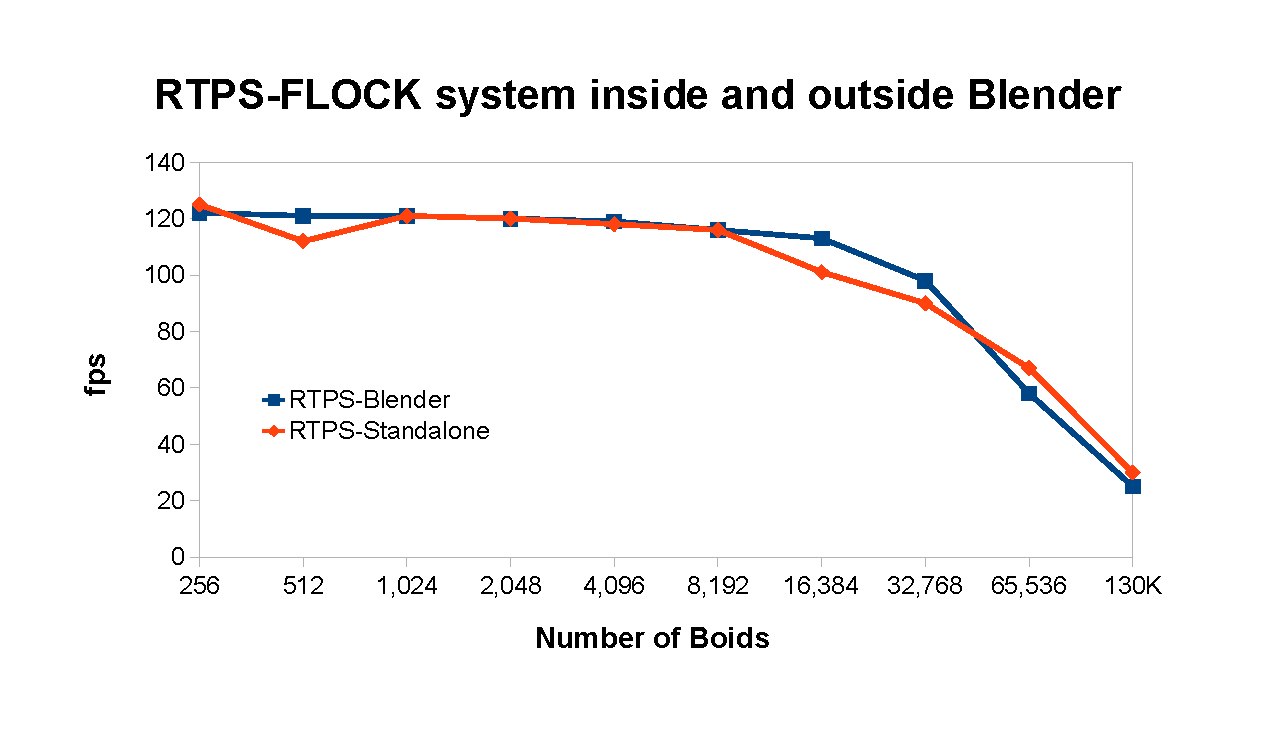
\includegraphics[scale=0.5]{../figures/RTPSvsRTPS.pdf}
	\end{column}
	\end{columns}

	%\begin{figure}[htbp]
	%\begin{center}
	%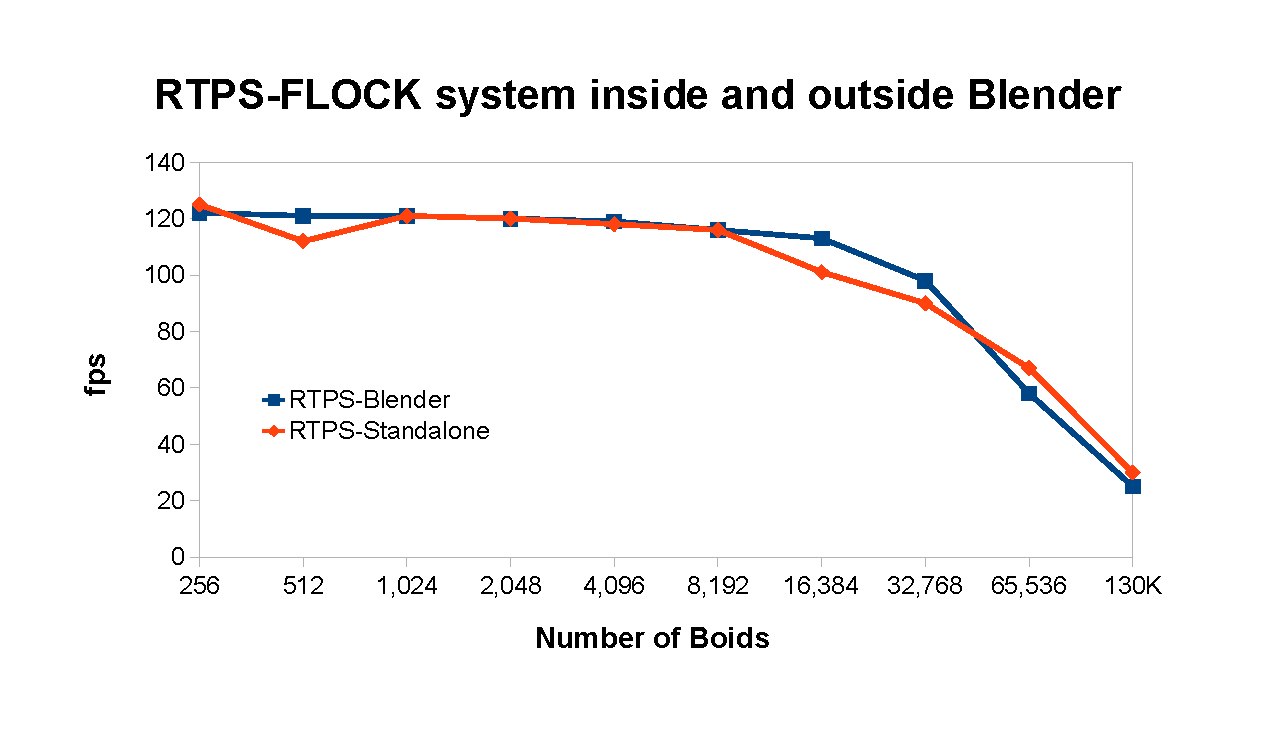
\includegraphics[scale=0.5]{../figures/RTPSvsRTPS.pdf}
	%\caption{Timings of RTPS-FLOCK system}
	%\end{center}
	%\end{figure}

\end{frame}

% RTPS Blender vs Blender
\begin{frame}{RTPS Blender vs Blender}

	\begin{columns}
	\begin{column}{2.25cm}
	\scriptsize
	~\textbf{Settings} \\
	~~maxBoids=256K \\
	~~maxSpeed = 2 \\
	~~searchRad = 1.5 \\
	~~minDist = 1\\
	~~w\_sep = 1 \\
	~~w\_align = 1 \\
	~~w\_coh = 1 \\
	~~w\_goal = 0 \\
	~~w\_avoid = 0 \\
	\end{column}
	
	\begin{column}{15cm}
	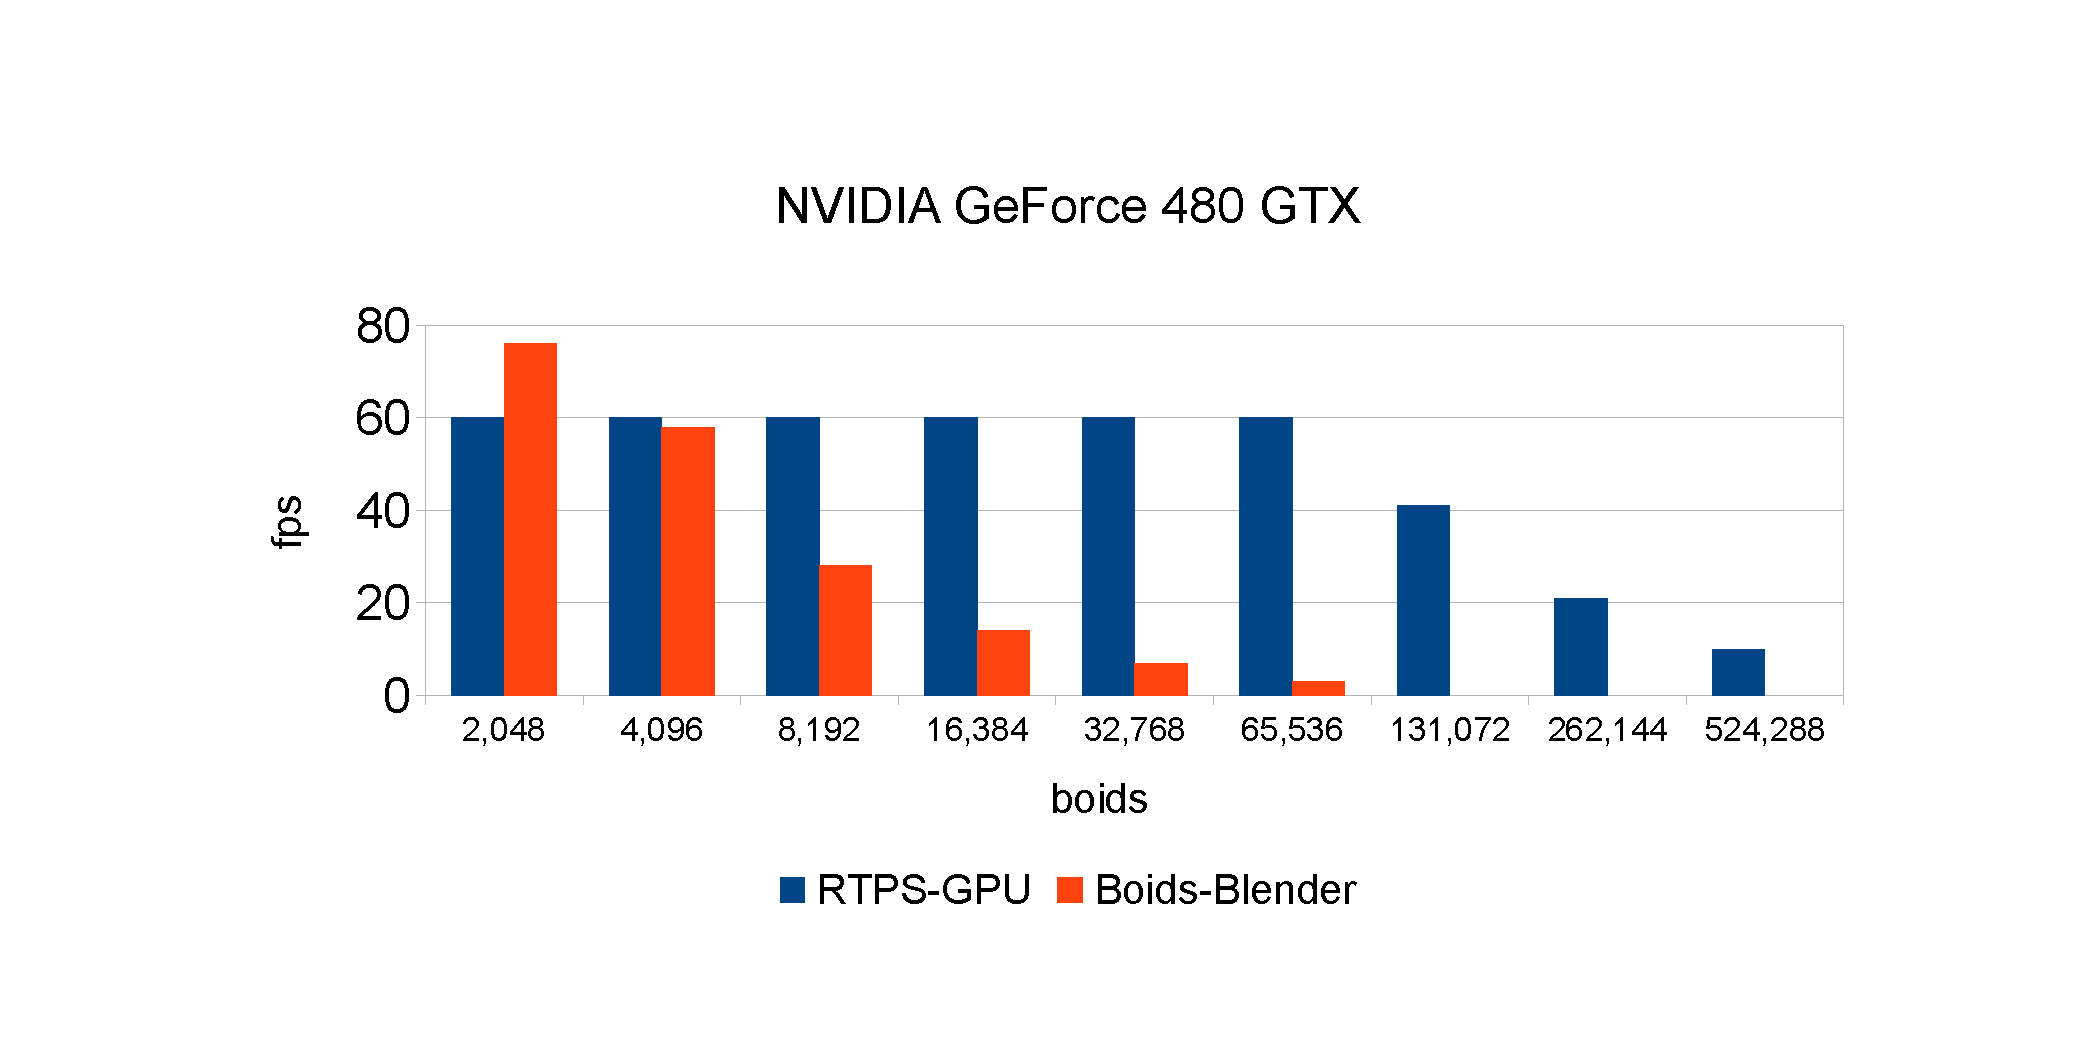
\includegraphics[scale=0.5]{../figures/benchmarks.pdf}
	\end{column}
	\end{columns}
	
	%\begin{figure}[htbp]
	%\begin{center}
	%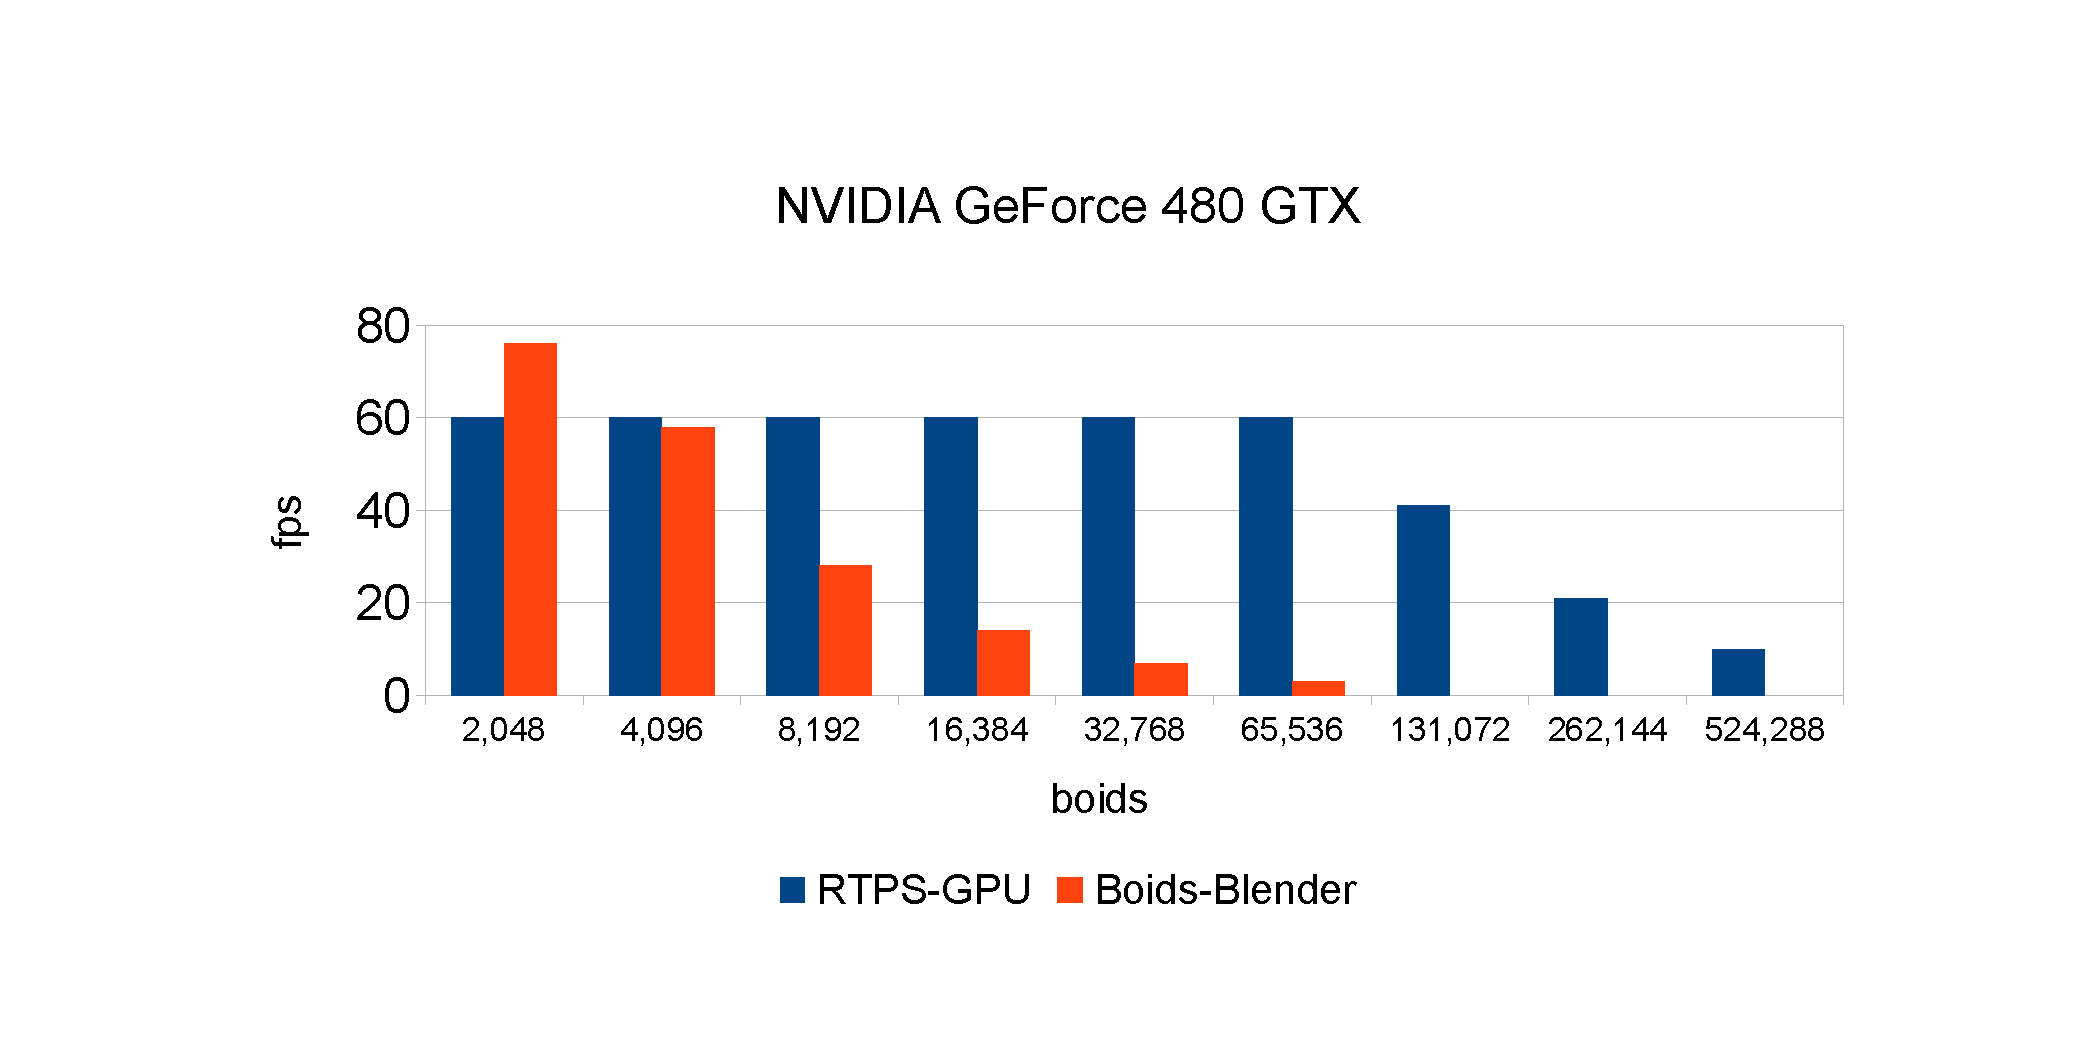
\includegraphics[scale=0.50]{../figures/benchmarks.pdf}
	%\caption{Timings of RTPS modifier and Blender Boids system}
	%\label{plot}
	%\end{center}
	%\end{figure}
\end{frame}

% speedup
\begin{frame}{Speedup} 
	\begin{figure}[htbp]
	\begin{center}
	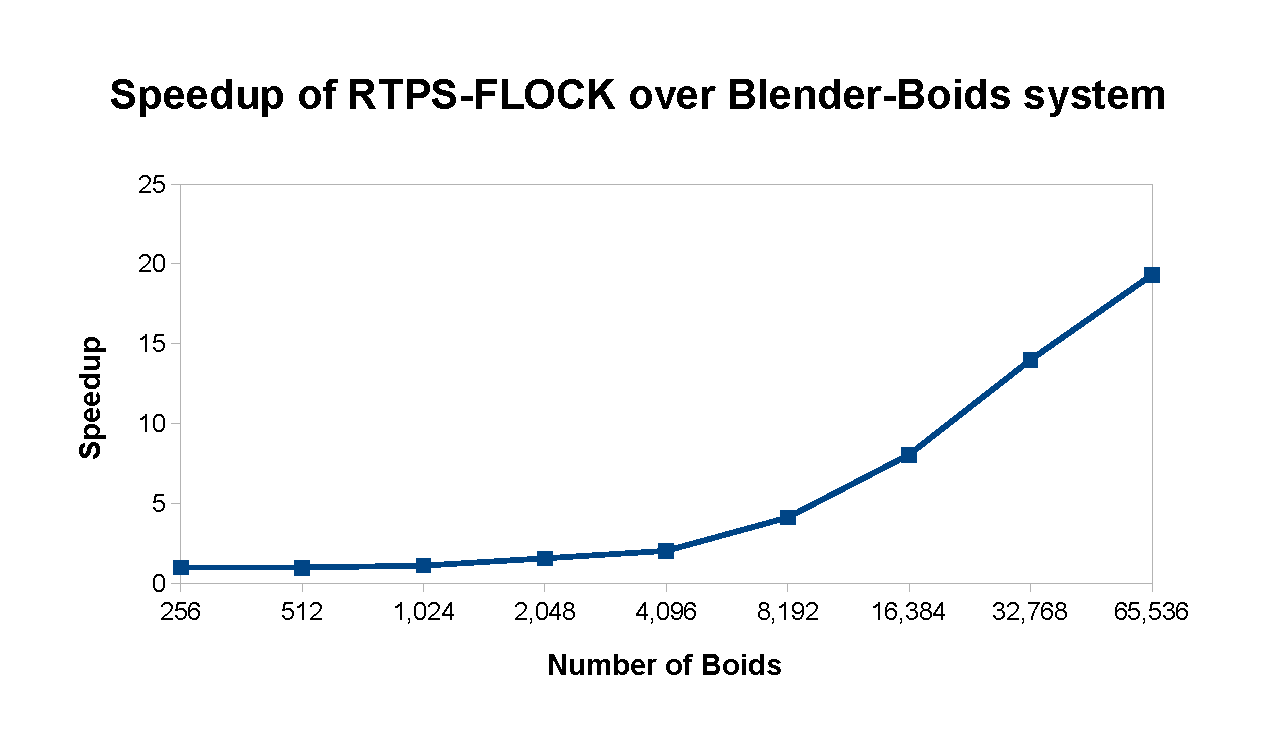
\includegraphics[scale=0.50]{../figures/speedup.pdf}
	%\caption{Speedup of the FLOCK system of the RTPS library over the Blender Boids system}
	\label{speedup}
	\end{center}
	\end{figure}
\end{frame}

% RTPS kernels
\begin{frame}{RTPS kernels}
	
	\begin{columns}
	\begin{column}{2.25 cm}
	\scriptsize
	~\textbf{Settings} \\
	~~maxBoids=256K \\
	~~maxSpeed = 2 \\
	~~searchRad = 1.5 \\
	~~minDist = 1 \\
	~~w\_sep = 1 \\
	~~w\_align = 1 \\
	~~w\_coh = 1 \\
	~~w\_goal = 0 \\
	~~w\_avoid = 0 \\
	\end{column}
	
	\begin{column}{15cm}
	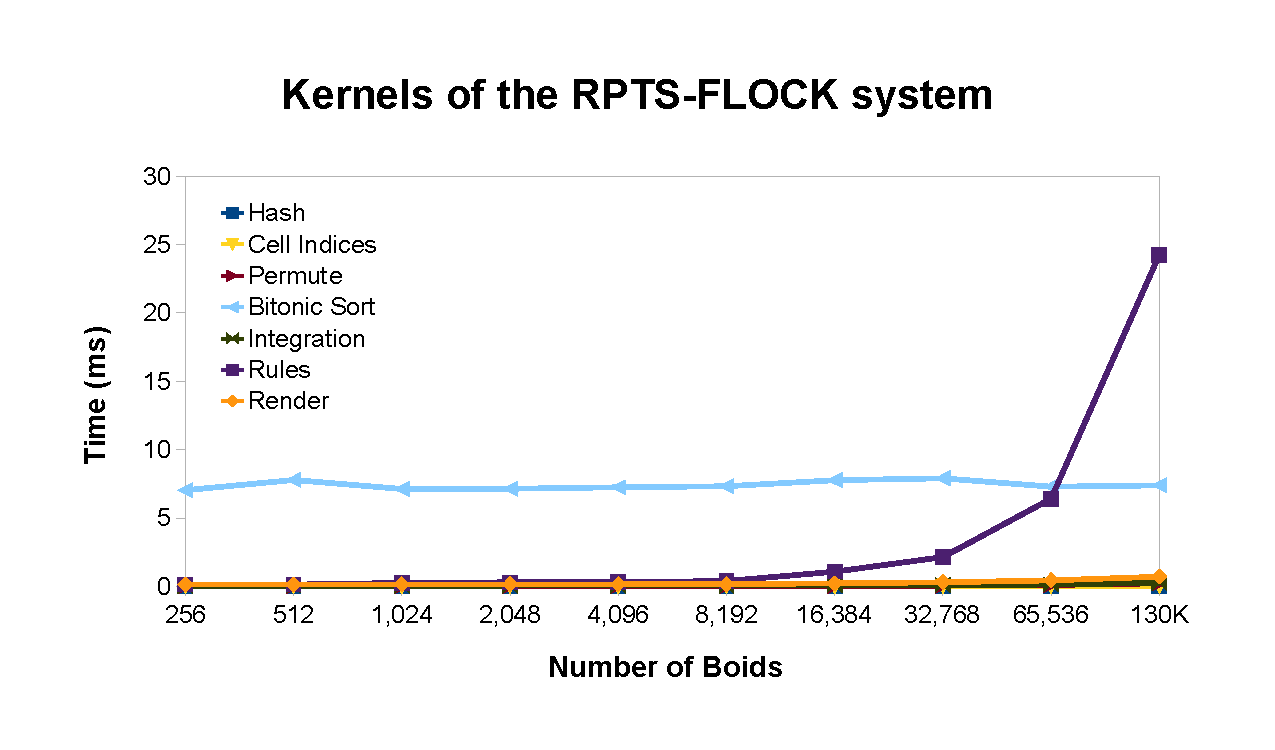
\includegraphics[scale=0.5]{../figures/kernelsPlot.pdf}
	\end{column}
	\end{columns}
	
	%\begin{figure}[htbp]
	%\begin{center}
	%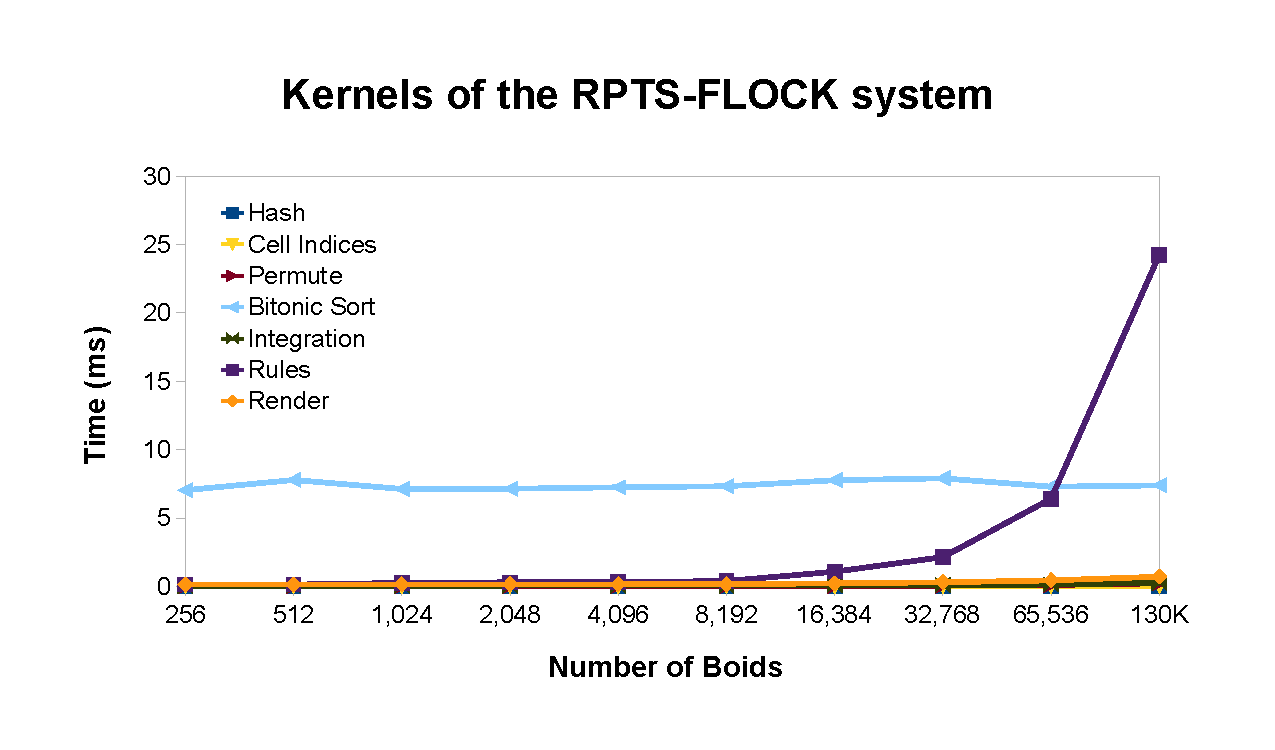
\includegraphics[scale=0.50]{../figures/kernelsPlot.pdf}
	%\caption{Timings for the kernels executed by the FLOCK system of RTPS}
	%\label{kernelBench}
	%\end{center}
	%\end{figure}
\end{frame}


%--------------------------------------------
% demos
%--------------------------------------------
\subsection{Demos}

% Symmetry
\begin{frame}{Symmetry Demo}
	\begin{figure}[htbp]
	\begin{center}
	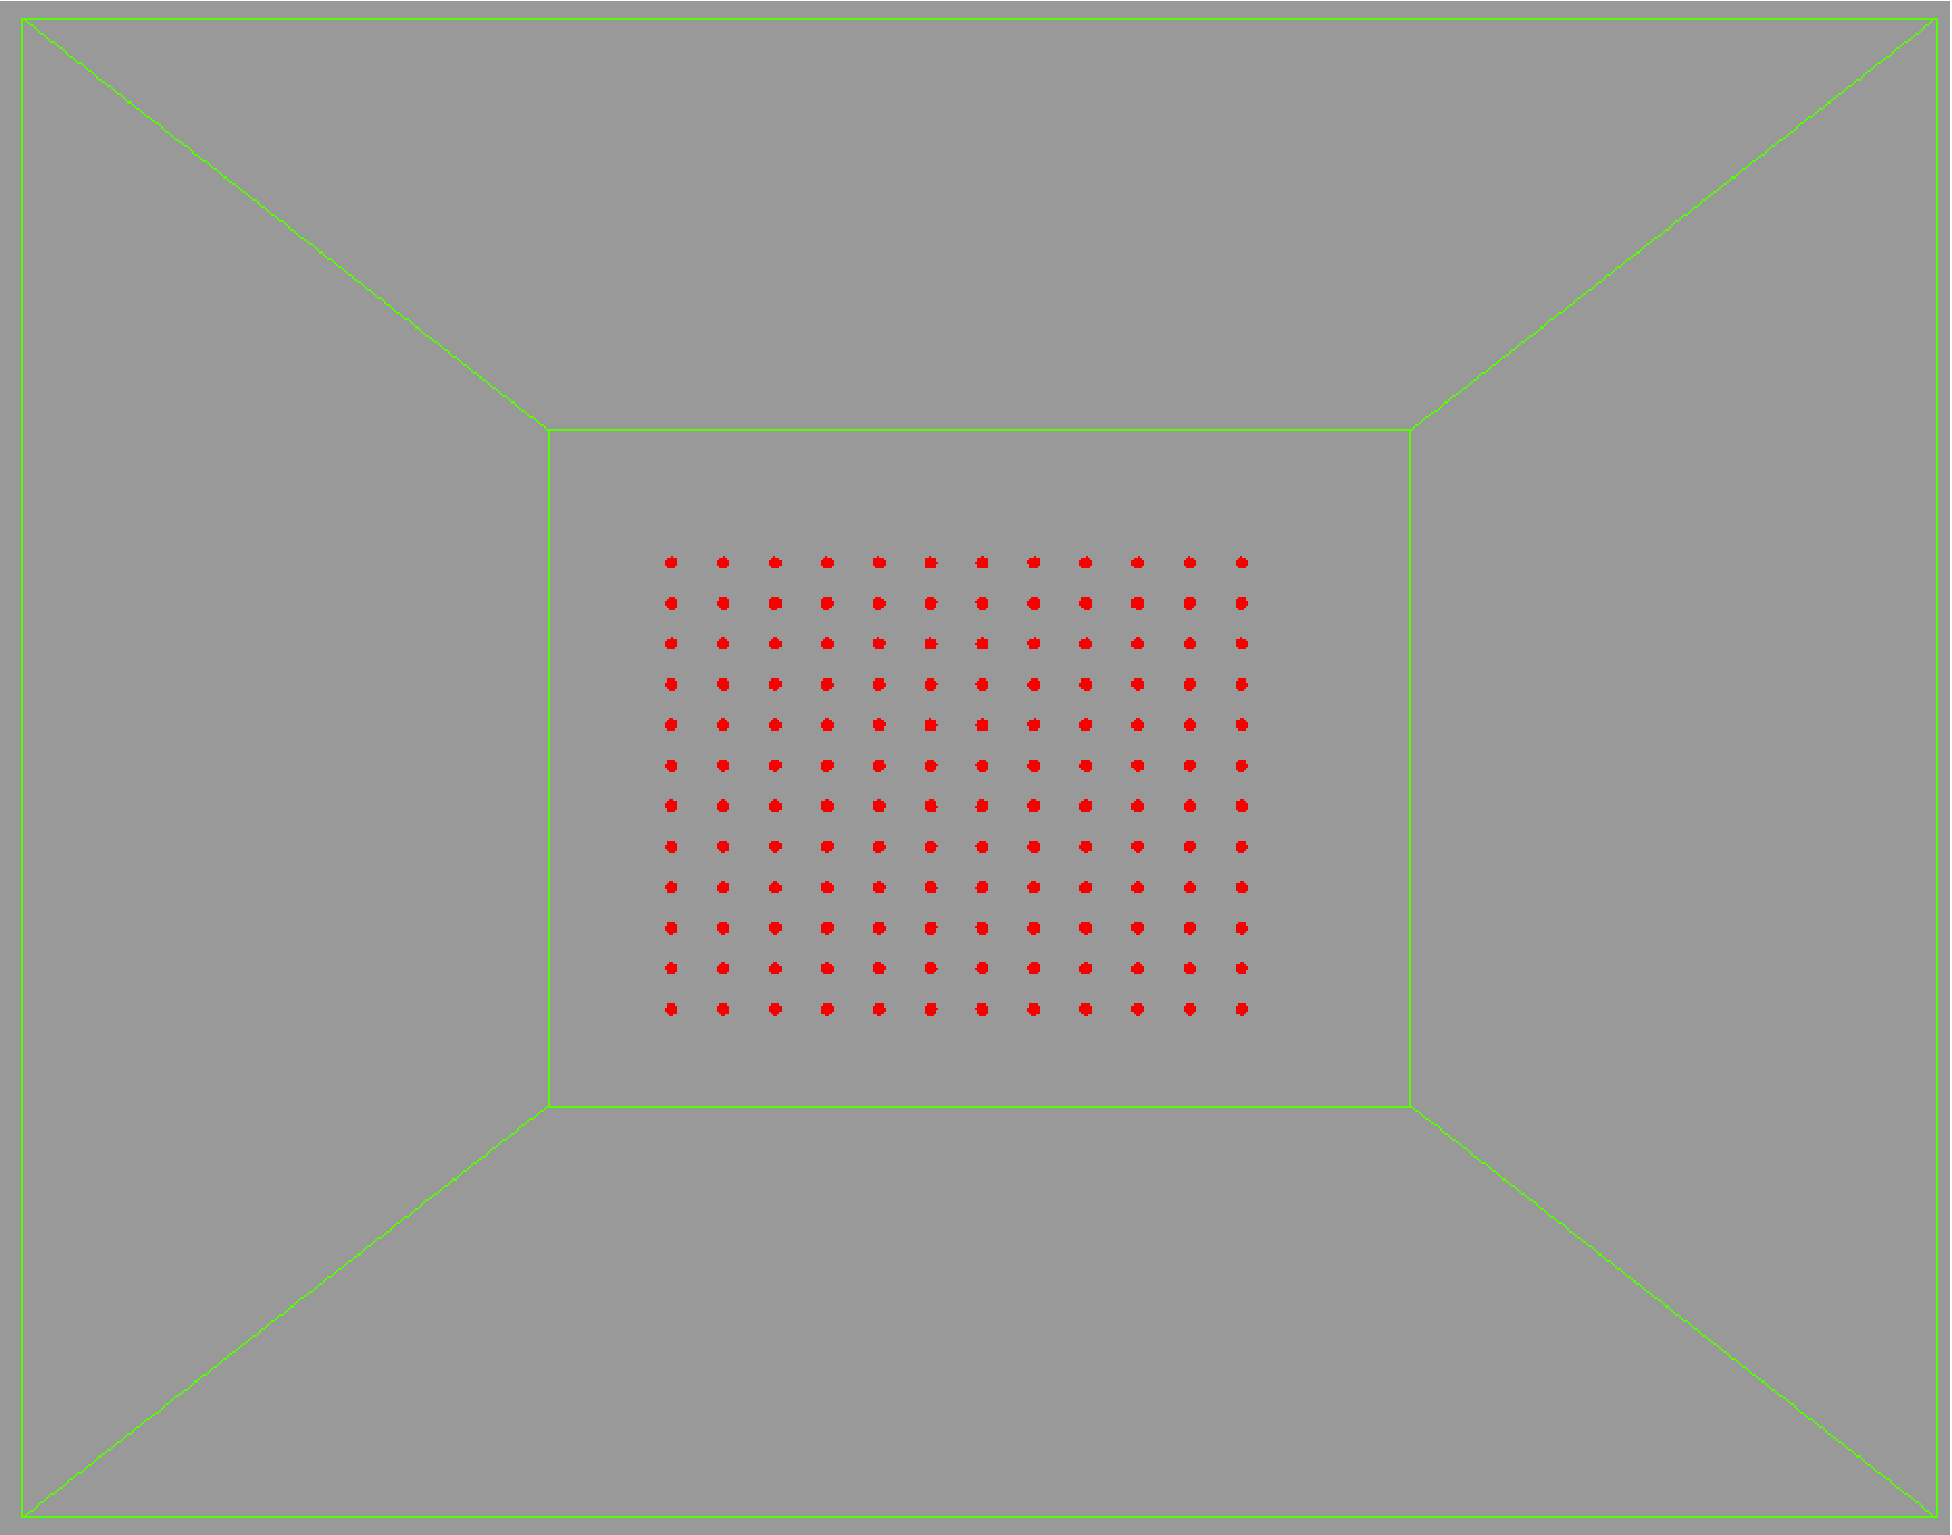
\includegraphics[scale=0.35]{../figures/align.pdf}
	\caption{Initial state of the boids}
	\label{alignRule}
	\end{center}
	\end{figure}
\end{frame}

\begin{frame}{Symmetry Demo: Separation}

	\begin{columns}
	\begin{column}{3.25 cm}
	\scriptsize
	~~\textbf{Settings} \\
	~~~maxSpeed = 2 \\
	~~~searchRad = 2 \\
	~~~minDist = 1.5 \\
	~~~w\_sep = 1 \\
	~~~w\_align = 0 \\
	~~~w\_coh = 0 \\
	~~~w\_goal = 0 \\
	~~~w\_avoid = 0 \\
	\end{column}
	
	\begin{column}{10cm}
	\includemovie[poster, text=(Separation Video), repeat]{6cm}{6cm}{../videos/video_separation.mpg}
	\end{column}
	\end{columns}

	%\begin{center}
  	%	\includemovie[poster, text=(Separation Video), repeat]{6cm}{6cm}{../videos/video_separation.mpg}
	%\end{center}
\end{frame}

\begin{frame}{Symmetry Demo: Cohesion}

	\begin{columns}
	\begin{column}{3.25 cm}
	\scriptsize
	~~\textbf{Settings} \\
	~~~maxSpeed = 2 \\
	~~~searchRad = 1 \\
	~~~minDist = 1 \\
	~~~w\_sep = 0 \\
	~~~w\_align = 0 \\
	~~~w\_coh = 1 \\
	~~~w\_goal = 0 \\
	~~~w\_avoid = 0 \\
	\end{column}
	
	\begin{column}{10cm}
	\includemovie[poster, text=(Cohesion Video), repeat]{6cm}{6cm}{../videos/video_cohesion.mpg}
	\end{column}
	\end{columns}
	
	%\begin{center}
  	%	\includemovie[poster, text=(Cohesion Video), repeat]{6cm}{6cm}{../videos/video_cohesion.mpg}
	%\end{center}
\end{frame}

% Goal Demo
\begin{frame}{Bees approaching their hive simulation}

	\begin{columns}
	\begin{column}{3.25 cm}
	\scriptsize
	~~\textbf{Settings} \\
	~~~maxSpeed = 2 \\
	~~~searchRad = 1.5 \\
	~~~minDist = 1 \\
	~~~w\_sep = 0.5 \\
	~~~w\_align = 0 \\
	~~~w\_coh = 0 \\
	~~~w\_goal = 1 \\
	~~~w\_avoid = 0 \\
	\end{column}
	
	\begin{column}{10cm}
	\includemovie[poster, text=(Goal Video), repeat]{6cm}{6cm}{../videos/video_goal.mpg}
	\end{column}
	\end{columns}
	
	%\begin{center}
  	%	\includemovie[poster, text=(Goal Video), repeat]{6cm}{6cm}{../videos/video_goal.mpg}
	%\end{center}
\end{frame}

% Blender
\begin{frame}{Crowding simulation}

	\begin{columns}
	\begin{column}{2 cm}
	\scriptsize
	~\textbf{Settings} \\
	~~maxSpeed=1\\
	~~searchRad=6\\
	~~minDist = 5 \\
	~~angVel = 1.5 \\
	~~w\_sep = 1 \\
	~~w\_align = 0.5 \\
	~~w\_coh = 0.5 \\
	\end{column}
	
	\begin{column}{11cm}
	\includemovie[poster, text=(Crowding Video), repeat]{10cm}{6cm}{../videos/video_crowd.mov}
	\end{column}
	\end{columns}
	
	%\begin{center}
  	%	\includemovie[poster, text=(Crowding Video), repeat]{10cm}{6cm}{../videos/video_crowd.mov}
	%\end{center}
\end{frame}

%--------------------------------------------
% conclusion
%--------------------------------------------
\section{Conclusion}
\begin{frame}{Conclusion}
	\begin{itemize}
		\item Using the RTPS library we were able to implement a flocking algorithm in OpenCL.
		\item A custom modifier was developed in Blender to call the RTPS library.
		\item The RTPS modifier can run a Boids system inside the Blender Game Engine.
		\item The performance of the RTPS modifier outperforms the Boids system of Blender.
	\end{itemize}
\end{frame}

%--------------------------------------------
% future work
%--------------------------------------------
\subsection{Future Work}
\begin{frame}{Future work}
	\begin{itemize}
		\item Expand the list of the implemented rules.
		\item Use Swarm Intelligence or Evolutionary Algorithm to select an optimized set of parameters for the system.
		\item Hybrid systems.
		\item Use Blender objects as emitter objects.
	\end{itemize}
\end{frame}

%--------------------------------------------
%acknowledgments
%--------------------------------------------
\subsection{Acknowledgements}

\begin{frame}{Acknowledgements}
	\begin{table}[htdp]
	\begin{center}
	\begin{tabular}{ccc}
	 & \textbf{Adviser} &\\
	 & Dr. Gordon Erlebacher &\\ 
	& &  \\
	& &  \\ 
	\textbf{Committee} 		&&  \textbf{Special Recognition}\\ 
	Dr. Xiaoqiang Wang 	&&  Ian Johnson\\ 
	Dr. Ming Ye 			&&  Andrew Young\\ 
	 					&&   Evan Bollig \\
	\end{tabular} 
	\end{center}
	\end{table}
\end{frame}

% questions
\begin{frame}
	\begin{center}
	\textbf{Questions?}
	\end{center}
\end{frame}


\end{document}